\documentclass[aoas, preprint]{imsart}
\RequirePackage{natbib}

%\long\def\authornote#1{%
%        \leavevmode\unskip\raisebox{-3.5pt}{\rlap{$\scriptstyle\diamond$}}%
%        \marginpar{\raggedright\hbadness=10000
%        \def\baselinestretch{0.8}\tiny
%        \it #1\par}}
%\newcommand{\ville}[1]{\authornote{NOTE TO SELF: #1}}

%\usepackage{amsthm,amsmath,natbib}
%\RequirePackage[colorlinks,citecolor=blue,urlcolor=blue]{hyperref}

% provide arXiv number if available:
%\arxiv{arXiv:0000.0000}

% put your definitions there:
\startlocaldefs
\endlocaldefs


\newcommand{\argmin}{\operatornamewithlimits{arg\ min}}
\newcommand{\argmax}{\operatornamewithlimits{arg\ max}}
\newcommand\ville[1]{{\color{red} #1 }}
%    \mymarginpar{\raggedright\hbadness=10000\tiny\it #1\par}}

%\usepackage[section]{placeins}
\usepackage{amsmath} 
\usepackage{times}
\usepackage{amsmath,amsthm,amssymb}
\usepackage{fancyhdr}
\usepackage{moreverb}
\usepackage{graphicx}
\usepackage{amssymb}
\usepackage{url}
\usepackage{multirow} 
\usepackage[boxed, section]{algorithm}
%\usepackage{algorithm}
\usepackage{algorithmic}
%\usepackage{cite}
\usepackage{multirow} 
\usepackage{rotating}
%\usepackage[margin=1.2in]{geometry}
\usepackage{geometry}
\usepackage{fix-cm}
\usepackage{subfigure}
\usepackage{bbm}
\usepackage{color} 
\usepackage{natbib}
\usepackage{xcolor,xparse}
\usepackage{xparse}
%\usepackage{setspace}
\usepackage{booktabs}
%\usepackage{subfig}
%\usepackage{caption, subcaption}



%\renewcommand{\baselinestretch}{1.2}
%\setlength{\topmargin}{-0.3in}
%\setlength{\textwidth}{6in}
%\setlength{\textheight}{8.5in}
%\setlength{\oddsidemargin}{0.25in}
%\setlength{\evensidemargin}{0.25in}
%\raggedbottom

%\doublespacing

\allowdisplaybreaks

% Math Macros.  It would be better to use the AMS LaTeX package,
% including the Bbb fonts, but I'm showing how to get by with the most
% primitive version of LaTeX.  I follow the naming convention to begin
% user-defined macro and variable names with the prefix "my" to make it
% easier to distiguish user-defined macros from LaTeX commands.
%
\newtheorem{mydef}{Definition}
\newcommand{\myN}{\hbox{N\hspace*{-.9em}I\hspace*{.4em}}}
\newcommand{\myZ}{\hbox{Z}^+}
\newcommand{\R}{\mathbb{R}}
\renewcommand{\P}{\mathbb{P}}
\newcommand{\E}{\mathbb{E}}
\newcommand{\logit}{\text{logit}}
\NewDocumentCommand{\framecolorbox}{oommm}
 {% #1 = width (optional)
  % #2 = inner alignment (optional)
  % #3 = frame color
  % #4 = background color
  % #5 = text
  \IfValueTF{#1}
   {%
    \IfValueTF{#2}
     {\fcolorbox{#3}{#4}{\makebox[#1][#2]{#5}}}
     {\fcolorbox{#3}{#4}{\makebox[#1]{#5}}}%
   }
   {\fcolorbox{#3}{#4}{#5}}%
 }



\newcommand{\myfunction}[3]
{${#1} : {#2} \rightarrow {#3}$ }

\newcommand{\myzrfunction}[1]
{\myfunction{#1}{{\myZ}}{{\myR}}}


\newcommand{\mysection}[1]
{\noindent {\bf {#1}}}

%%%%%% Begin document with header and title %%%%%%%%%

\begin{document}
\begin{frontmatter}
% "Title of the paper"
\title{Probability Aggregation: Dynamic Hierarchical Modeling of Sparse Expert Beliefs}
\runtitle{Dynamic Hierarchical Modeling of Sparse Expert Beliefs}

% indicate corresponding author with \corref{}
% \author{\fnms{John} \snm{Smith}\corref{}\ead[label=e1]{smith@foo.com}\thanksref{t1}}
% \thankstext{t1}{Thanks to somebody} 
% \address{line 1\\ line 2\\ printead{e1}}
% \affiliation{Some University}


%\begin{aug}
%  \author{\fnms{First}  \snm{Author}\corref{}\thanksref{t2}\ead[label=e1]{first@somewhere.com}},
%  \author{\fnms{Second} \snm{Author}\ead[label=e2]{second@somewhere.com}}
%  \and
%  \author{\fnms{Third}  \snm{Author}%
%  \ead[label=e3]{third@somewhere.com}%
%  \ead[label=u1,url]{http://www.foo.com}}
%
%  \thankstext{t2}{Footnote to the first author with the `thankstext' command.}
%
%  \runauthor{F. Author et al.}
%
%  \affiliation{Some University and Another University}
%
%  \address{Address of the First and Second authors,\\ 
%          \printead{e1,e2}}
%
%  \address{Address of the Third author,\\
%          \printead{e3,u1}}
%
%\end{aug}

\begin{aug}
\author{\fnms{Ville A.} \snm{Satop\"a\"a}\corref{}\ead[label=e1]{satopaa@wharton.upenn.edu}},
\author{\fnms{Shane T.} \snm{Jensen}\ead[label=e3]{stjensen@wharton.upenn.edu}},
\author{\fnms{Lyle H.} \snm{Ungar}\ead[label=e2]{ungar@cis.upenn.edu}},
\author{\fnms{Barbara A.} \snm{Mellers}\ead[label=e4]{mellers@wharton.upenn.edu}},
\and
\author{\fnms{Phil E.} \snm{Tetlock}\ead[label=e5]{tetlock@wharton.upenn.edu}}

\runauthor{Satop\"a\"a et al.}

 \affiliation{Department of Statistics, The Wharton School of the University of Pennsylvania\\   \printead{e1,e3}}
 \affiliation{Department of Computer and Information Science, University of Pennsylvania\\ \printead{e2}}
 \affiliation{Department of Psychology, University of Pennsylvania\\ \printead{e4,e5}}
 \address{Philadelphia, PA 19104- 6340, USA\\  \printead{e1}}
  
\end{aug}

\begin{abstract}
Most subjective probability aggregation procedures use a single probability judgement from each expert, even though it is common for experts studying real problems to update their probability estimates over time.  This paper makes an advance towards unexplored areas of probability aggregation by considering a dynamic context in which experts are allowed to update their beliefs at random intervals. The updates are assumed to occur very infrequently, resulting into a highly sparse dataset that cannot be modeled by standard time-series procedures. In response to the lack of appropriate methodology, this paper presents a hierarchical model that takes into account the expert's level of self-reported expertise and produces aggregate probabilities that are sharp and well-calibrated both in- and out-of-sample. The model is demonstrated on a real-world dataset that includes over 2,300 experts making multiple probability forecasts on different subsets of 166 international political events. 
\end{abstract}


\begin{keyword}
\kwd{Probability Aggregation}
\kwd{Dynamic Linear Model}
\kwd{Hierarchical Modeling}
\kwd{Expert Forecast}
\kwd{Subjective Probability}
\kwd{Bias Estimation}
\kwd{Calibration}
\kwd{Time Series}
\end{keyword}
\end{frontmatter}



\section{Introduction}
\label{intro}
Individual experts can differ radically from one another in their abilities to assess probabilities of future events. Their probability assessments are often evaluated and compared in regards to \textit{calibration} that measures how closely the frequency of occurrence of the events agree with the given probabilities. For instance, the proportion of occurred events is 60\% for all those events for which a well-calibrated expert assessed a probability of 0.60. Even though several experiments have been conducted to show that experts are generally poorly calibrated (see, e.g., \citet{cooke1991experts, shlyakhter1994quantifying}), relative differences can occur among different types of experts. In particular, \citet{wright1994coherence} argue that a higher level of self-reported expertise can be associated with better calibration. 

Calibration by itself, however, is not sufficient for a useful probability assessment. To see this, consider a relatively stationary process, such as rain on different days in some geographic region, whose empirical frequency of occurrence in the last 10 years is 45\%. In this setting an expert can assess a constant probability of 0.45 and be well-calibrated. This assessment, however, can be made without any subject-matter expertise or special training. For this reason the long-term frequency is often considered as the baseline probability -- a naive assessment that provides the decision-maker very little extra information. Therefore a consulting expert should aim to make probability assessments that are as far from the baseline as possible. The extent to which his probabilities differ from the baseline is measured with an important attribute called \textit{sharpness} (\citet{gneiting2008rejoinder, winkler2008comments}). If the expert is both sharp and well-calibrated, he is able to forecast the behavior of the process with high certainty and accuracy. From the decision-maker's perspective his advice is highly useful as it involves much information and very little risk. Therefore, to summarize, useful probability estimation should aim to maximize sharpness subject to calibration (see, e.g., \citet{raftery2005using, murphy1987general}). This is a well-defined goal that has led to a wide range of novel and insightful observations in probability forecasting. 

One such observation is related to the aggregation of multiple probabilities. There is strong empirical evidence that bringing together the strengths of different experts by combining their probability forecasts into a single consensus, known as the \textit{crowd belief},  results in better predictive performance. Being motivated by the long list of applications of probability forecasts, including medical diagnosis (\citet{wilson1998prediction, pepe2003statistical}, political and socio-economic foresight (\citet{tetlock2005expert}), and meteorology (\citet{sanders1963subjective, vislocky1995improved, baars2005performance}), researchers have proposed many different approaches to combining probability forecasts (see, e.g., \citet{Ranjan08, satopaa} for some recent studies, and \citet{Genest, Wallsten97evaluatingand, clemen2007aggregating, primo2009calibration} for a comprehensive overview). The general focus, however, has been on developing one-time aggregation procedures that consult the expert's advice only once before the event resolves. 

Consequently, many areas of probability aggregation still remain rather unexplored. For instance, consider an investor aiming to assess whether a stock index will finish trading above some threshold on a given date. In order to maximize his overall predictive accuracy, he may consult a group of experts repeatedly over a period of time and adjust his estimate of the aggregate probability accordingly. Since the experts are allowed to update their probability assessments, the aggregation should be performed by taking into account the temporal correlation in their advice. Many standard time-series procedures could be used to perform this aggregation as long as the experts update their advice consistently on a daily basis. 

This paper adds another layer of complexity by assuming a heterogeneous set of experts, most of whom only make one or two probability assessments over the hundred or so days before the event resolves. This means that the decision-maker faces a different group of experts  every day, with only a few experts returning later on for a second round of advice. The problem at hand is therefore strikingly different from many time-series estimation problems, where one has an observation at every time point -- or almost every time point. As a result, standard time-series procedures like ARIMA (see, e.g., \citet{mills1991time}) are not directly applicable to our setting. In response to the lack of appropriate modeling procedures, this paper introduces a time-series model that incorporates self-reported expertise and captures a sharp and well-calibrated estimate of the crowd belief. The model is highly interpretable and can be used for:
\begin{itemize}
\item the analysis of group-level under- and overconfidence across different levels of self-reported expertise,
%\item confidence bands for the crowd belief,
\item accurate probability forecasts, and
\item many question-specific quantities that have easy interpretations and can be used to gain novel insight in the social sciences. 
\end{itemize}

The paper begins with a description of our probability forecasting data that were collected by asking over 2,300 experts to give probability forecasts and to self-assess their level of expertise on a subset of 166 geopolitical binary events. After summarizing the dataset, the paper introduces a dynamic hierarchical model for capturing the crowd belief. The model is estimated in a two-step procedure: first, a sampling step produces constrained parameter estimates via Gibbs sampling (see \citet{geman1984stochastic} for the original introduction of Gibbs sampling); second, a calibration step transforms these estimates to their unconstrained equivalents via a one-dimension optimization procedure. An extension of this model to polychotomous outcomes is briefly discussed before model evaluation. The first evaluation section uses synthetic data to study the accuracy to which the two-step procedure is able to estimate parameter values. The second evaluation section illustrates different aspects of the model by applying it to our real-world probability forecasting data. The paper concludes with a discussion on future research directions and model limitations.

\section{Geopolitical Forecasting Data}
\label{data}

\begin{table}
\begin{center}
\begin{tabular}{c c c c c c c c }
\hline
Statistic & Min. & $Q_1$ & Median & Mean & $Q_3$ & Max.\\ \hline
\# of Days a Question is Active  & 4 &  35.6 &  72.0 & 106.3 & 145.20 & 418 \\
\# of Experts per Question & 212 &   543.2 &  693.5 &  783.7 &  983.2 & 1690\\ 
\# Forecasts given by each Expert on a Question & 1 &  1.0 &   1.0  &  1.8 &  2.0 & 131 \\
\# Questions participated by an Expert & 1 &  14.0 &   36.0  &  55.0 &  90.0 & 166 \\ \hline
\end{tabular}
\caption{Five-number summaries of our real-world data.
%: \textit{\# of Days Active} represents the number of days that the experts were given to update their forecast before the correct answer was revealed; \textit{\# of Experts per Problem } denotes the number of experts participating in a question; \textit{\# Forecasts given by each Expert on a Problem} gives the number of forecasts for a question made by an active expert; \textit{\# Problems participated by an Expert} represents the number of different questions a given expert participated in.
}
\label{DataStats}
\end{center}
\end{table}

\begin{table}
\begin{center}
\begin{tabular}{c c c c c c c c }
\hline
Expertise Level & 1 & 2 & 3 & 4 & 5\\
Frequency (\%) & 25.3 & 30.7 & 33.6 &  8.2 &  2.1 \\\hline
\end{tabular}
\caption{Frequencies of the self-reported expertise (1 = Not At All Expert and 5 = Extremely Expert) levels across all the 166 questions in our real-world data.}
\label{ExpertiseTable}
\end{center}
\end{table}



The data collection began with a recruitment of 2,365 experts ranging from graduate students to political science faculty and practitioners. The recruiting was made from professional societies, research centers, alumni associations, science bloggers, and word of mouth. Requirements included at least a Bachelor's degree and completion of psychological and political tests that took roughly two hours. These measures assessed cognitive styles, cognitive abilities, personality traits, political attitudes, and real-world knowledge. The experts were asked to give probability forecasts (to the second decimal point) and to self-assess their level of expertise (on a 1-to-5 scale with 1 = Not At All Expert and 5 = Extremely Expert) on a number of 166 geopolitical binary events taking place between September 29, 2011 and May 8, 2013. Each question was active for a period of time during which the participating experts were allowed to update their forecasts as frequently as they liked without being penalized. The experts knew that their probability estimates would be assessed for accuracy using Brier scores\footnote{The Brier score is the squared distance between the probability forecast and the event indicator that equals 1.0 or 0.0 depending on whether the event happened or not, respectively. See \citet{Brier} for the original introduction.}. This incentivized them to report their true beliefs instead of attempting to game the system (\citet{winkler1968good}). In addition to receiving \$150 for meeting minimum participation requirements that did not depend on prediction accuracy, the experts received status rewards for their performance via leader-boards displaying Brier scores for the top 20 experts. Since a typical expert participated only in a small subset of the 166 questions, the experts are considered indistinguishable conditional on the level of self-reported expertise.


The experts made updates on a very infrequent basis. An expert gave, on average, only 0.016 forecasts per day; that is, a forecast in about every 63 days. The average group-level response rate was around 13.5 forecasts per day. Given that the group of experts is large and diverse, the data is very sparse. Tables \ref{DataStats} and \ref{ExpertiseTable} provide more relevant summary statistics on the data. Notice that the distribution of the self-reported expertise is skewed to the right and that some questions remained active longer than others.  For more details on the data and its collection see \citet{ungar2012good}.

\begin{figure}[h!]
\vspace{-2em}
\centering
\hspace*{0em} 	
\includegraphics{Figures/LegendExamplePlot} % requires the graphicx package
\vspace{-3.5em}

\hspace{-0.5em}
\subfigure[\textit{Will the expansion of the European bailout fund be ratified by all 17 Eurozone nations before 1 November 2011?}]{
\hspace*{-1em}  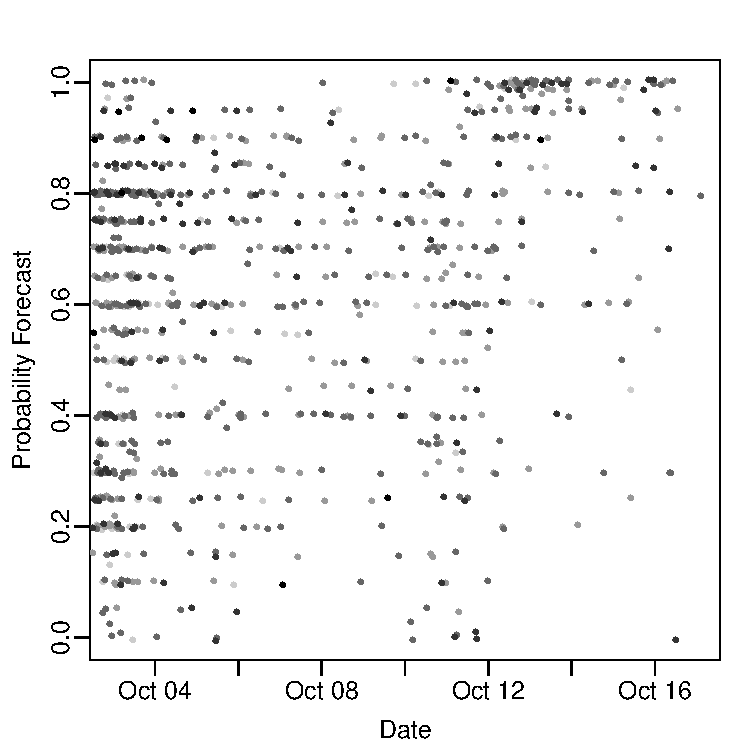
\includegraphics[width= 0.49\textwidth]{Figures/ExamplePlot1}
\label{Example1}
} \hspace{0.5em}
\subfigure[\textit{Will the Nikkei 225 index finish trading at or above 9,500 on 30 September 2011?}]{
\hspace*{-1em}  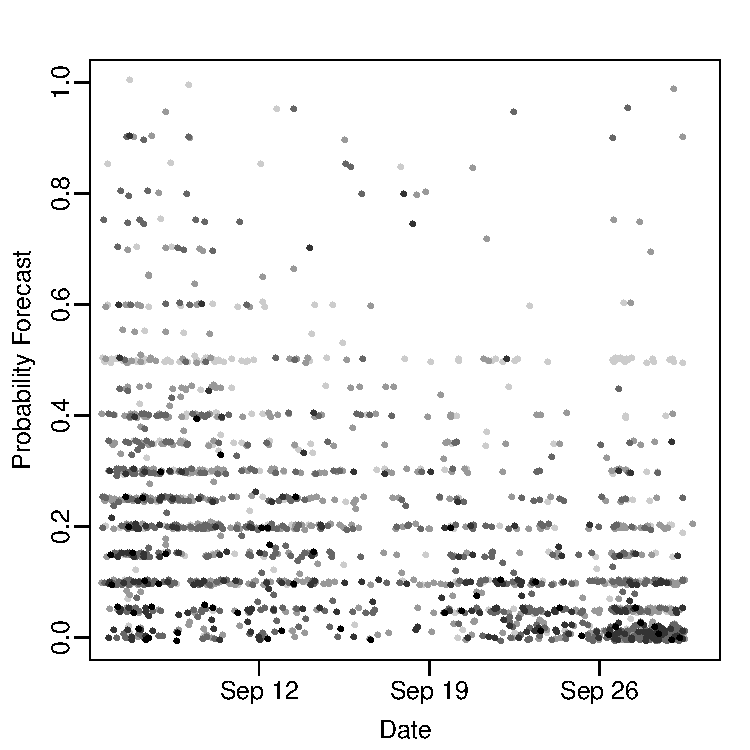
\includegraphics[width= 0.49\textwidth]{Figures/ExamplePlot2}
\label{Example2}
}

\caption[Optional caption for list of figures]{Scatterplots of the probability forecasts given for two questions in our dataset. The shadings represents the self-reported expertise of the expert who provided the probability forecast.}
\label{ExamplePlots}
\end{figure}



To illustrate the nature of the data with some concrete examples, Figures \ref{Example1} and \ref{Example2} show scatterplots of the probability forecasts given for (a) \textit{Will the expansion of the European bailout fund be ratified by all 17 Eurozone nations before 1 November 2011?}, and (b) \textit{Will the Nikkei 225 index finish trading at or above 9,500 on 30 September 2011?}. The points have been jittered slightly to make overlaps visible. The darkness of the points is positively associated with the self-reported expertise. Given that the European bailout fund was ratified before November 1, 2011 and that the Nikkei 225 index finished trading at around 8,700 on September 30, 2011, the general trend of the probability forecasts tends to converge towards the correct answers. The individual experts, however, disagree rather strongly, with the disagreement persisting even near the closing dates of the questions. 







\section{Model}
\label{model}
Let $p_{i,t,k} \in (0,1)$ be the probability forecast given by the $i$th expert at time $t$ for the $k$th question, where $i = 1, \dots, I_k$, $t = 1, \dots, T_k$, and $k = 1, \dots, K$. Denote the logit-probabilities with 
\begin{eqnarray*}
Y_{i,t,k} = \logit(p_{i,t,k}) = \log \left( \frac{p_{i,t,k}}{1-p_{i,t,k}}\right) \in \R
\end{eqnarray*}
and collect the logit-probability forecasts given for question $k$ at time $t$ into a vector $\boldsymbol{Y}_{t,k} = [Y_{1,t,k}\ Y_{2,t,k}\ \dots\ Y_{I_{k},t,k}]^T$. Partition the experts into $J$ groups based on some individual feature, such as self-reported expertise, with each group sharing a common multiplicative bias term $b_{j} \in \R$ for $j = 1, \dots, J$. Collect these bias terms into a bias vector $\boldsymbol{b} = [b_{1}\ b_{2}\ \dots\ b_{J}]^T$. Let $\boldsymbol{M}_k$ be a $I_k \times J$ matrix denoting  the group-memberships of the experts in question $k$; that is, if the $i$th expert participating in the $k$th question belongs to the $j$th group, then the $i$th row of $\boldsymbol{M}_k$ is the $j$th standard basis vector $\boldsymbol{e}_j$. The bias vector $\boldsymbol{b}$ does not include a subindex because it is considered shared among all the $K$ questions. To secure model identifiability, it is sufficient to share only one of the elements of $\boldsymbol{b}$ among the questions. This element defines a baseline under which it is possible to estimate the remaining $J-1$ bias terms separately within each of the questions. In this paper, however, the entire vector $\boldsymbol{b}$ is shared because some of the questions in our real-world data set involve very few experts with the highest level of self-reported expertise. Under this notation, the model for the $k$th question can be expressed as 
\begin{eqnarray}
\boldsymbol{Y}_{t, k} &=&  \boldsymbol{M}_k \boldsymbol{b} X_{t, k} + \boldsymbol{v}_{t, k} \label{observedpr} \\
X_{t, k} &=& \gamma_k X_{t-1, k} + w_{t, k} \label{hiddenpr}\\
X_{0,k} &\sim& \mathcal{N}(\mu_0, \sigma^2_0) \nonumber
\end{eqnarray}
where Equation (\ref{observedpr}) denotes the observed process and Equation (\ref{hiddenpr}) shows the hidden process that is driven by the constant $\gamma_k \in \R$. The error terms are independent and identically distributed normal random variables with mean zero
\begin{eqnarray*}
\boldsymbol{v}_{t, k} | \sigma^2_k &\stackrel{i.i.d.}{\sim}& \mathcal{N}_{I_k}(\boldsymbol{0}, \sigma^2_k \boldsymbol{I}_{I_k})\\
w_{t, k} | \tau^2_k &\stackrel{i.i.d.}{\sim}& \mathcal{N}(0, \tau^2_k),
\end{eqnarray*}
and $(\mu_0, \sigma_0^2) \in (\R, \R^+)$ are hyper-parameters chosen \textit{a priori}. 

The hidden state $X_{t,k}$ represents the logit-probability for the $k$th event given all the information available up to and including time $t$. To make this more specific, let $Z_k \in \{0, 1\}$ indicate whether the event associated with the $k$th question happened $\left(Z_k = 1\right)$ or did not happen $\left(Z_k = 0\right)$. If $\{\mathcal{F}_{t,k}\}_{t=1}^{T_k}$ is a filtration representing the information available up to and including a given time point, then $\E[Z_k | \mathcal{F}_{t,k}] = \P(Z_k = 1| \mathcal{F}_{t,k}) = \logit^{-1}(X_{t,k})$. It is reasonable to assume that this probability forecast 
%that makes uses all available information and hence is equivalent to $\logit^{-1}(X_{t,k})$ 
%an expert, who has access to all available information and reports $\logit^{-1}(X_{t,k})$ as the probability forecast, 
maximizes sharpness subject to calibration, where calibration and sharpness are understood as follows:
\begin{mydef}
A probability forecast $p$ for the $k$th question is calibrated if $\P(Z_k = 1 | p) = \E[Z_k | p] = p$ almost surely (see, e.g., \citet{murphy1987general}).
\end{mydef}
\begin{mydef}
A probability forecast $p$ is sharper than a probability forecast $q$ if $\E[(p-p_0)^2] > \E[(q-p_0)^2]$, where $p_0$ is the baseline probability for the $k$th question (see, e.g., \citet{ranjan2009combining}). 
\end{mydef}
\noindent
Even though it is unlikely that any single expert has access to all the available information, a large and diverse group of experts may share a considerable portion of the available information. The collective wisdom of the group therefore provides an attractive proxy for $\mathcal{F}_{t,k}$. 


Since the experts may believe in false information, hide their true beliefs for ethical bases, or be biased for many other reasons, their probability assessments should be aggregated via a model that can detect potential bias, separate signal from noise, and use the collective opinion to estimate $X_{t,k}$. In our model the experts are assumed to be, on average, a multiplicative constant $\boldsymbol{b}$ away from $X_{t,k}$. Therefore an individual element of $\boldsymbol{b}$ can be interpreted as a group-specific \textit{systematic bias} that labels the group either as over-confident $\left( b_j \in (1, \infty)\right)$ or as under-confident $\left(b_j \in (0,1)\right)$.  Due to the high sparsity of our data, estimating a bias term separately for each expert is not possible. See Section \ref{ExpertBias} for an analysis and discussion on the bias terms. Any other deviation from $X_{t,k}$ is considered \textit{random noise}. This noise is measured in terms of $\sigma^2_k$ and can be assumed to be caused by momentary over-optimism (or pessimism), false beliefs, or other misconceptions. 
 
 The \textit{random fluctuations} in the hidden process are measured in terms of $\tau^2_k$ and are assumed to represent changes or shocks to the underlying circumstances that ultimately decide the outcome of the event. The \textit{systematic component} $\gamma_k$ allows the model to incorporate a constant signal stream that drifts the hidden process to infinity (when $\gamma_k \in (1, \infty)$) or zero (when $\gamma_k \in (0, 1)$). If the uncertainty in the question diminishes as the current time point $t$ approaches $T_k$, the hidden process drifts to infinity. Alternatively, the hidden process can drift to zero in which case any available information about the target event does not improve predictive accuracy. Since each of the $K$ questions in our dataset was resolved within a pre-specified timeframe, $\gamma_k$ is expected to fall within the interval $(1, \infty)$ for all $k = 1, \dots, K$. 
 

\section{Model Estimation}
\label{identifiability}


The main challenge is to capture a well-calibrated estimate of the hidden process without sacrificing the interpretability of our model. This section introduces a two-step procedure, called \textit{Sample-And-Calibrate} (SAC), that achieves this goal in a flexible and efficient manner: the first step estimates the model parameters under a constraint (\textit{Sampling Step}), and the second step performs a one-dimension optimization procedure to transform the constrained estimates into their unconstrained counterparts (\textit{Calibration Step}). 


\subsection{Sampling Step}
\label{sampling_step}
Since $\left(a \boldsymbol{b}, X_{t,k}/a, a^2 \tau_k^2\right) \neq \left(\boldsymbol{b}, X_{t,k}, \tau_k^2\right)$ for any $a > 0$ yield the same  likelihood for $\boldsymbol{Y}_{t,k}$, the model as described by Equations (\ref{observedpr}) and (\ref{hiddenpr}) is not identifiable. As a result, the parameter estimates tend to drift during the sampling process. A well-known solution is to choose one of the elements of $\boldsymbol{b}$, say $b_3$, as the reference point and fix $b_3 = 1$.  Denote the constrained version of the model by
\begin{eqnarray*}
\boldsymbol{Y}_{t, k} &=&  \boldsymbol{M}_k \boldsymbol{b} (1) X_{t, k}(1)+ \boldsymbol{v}_{t, k}\\
X_{t, k}(1) &=& \gamma_k(1) X_{t-1, k}(1) + w_{t, k}\\
\boldsymbol{v}_{t, k} | \sigma^2_k(1) &\stackrel{i.i.d.}{\sim}& \mathcal{N}_{I_k}(\boldsymbol{0}, \sigma^2_k(1) \boldsymbol{I}_{I_k})\\
w_{t, k} | \tau^2_k(1) &\stackrel{i.i.d.}{\sim}& \mathcal{N}\left(0, \tau^2_k(1)\right),
\end{eqnarray*}
where the trailing input parameter emphasizes the constraint $b_{3} = 1$. Since this version is identifiable, estimates of the model parameters can be obtained. Denote the estimates by placing a hat on the parameter symbol. For instance, $\hat{\boldsymbol{b}}(1)$ and $\hat{X}_{t, k}(1)$ represent the estimates of $\boldsymbol{b}(1)$ and $X_{t, k}(1)$, respectively. These estimates are found via Gibbs sampling that only makes use of standard distributions. See Appendix \ref{appendix} for the technical details of the sampling step, and, e.g., \citet{gelman2003bayesian} for a discussion on the general principles of Gibbs sampling. 



\subsection{Calibration Step}
\label{calibration_step}
Since the model parameters can be estimated by fixing $b_3$ to any constant, the next step is to search for the constant that gives an optimally sharp and calibrated estimate of the hidden process.  This section introduces an efficient procedure that finds the optimal constraint without requiring any additional runs of the sampling step. First, assume that parameter estimates  $\hat{\boldsymbol{b}}(1)$ and $\hat{X}_{t, k}(1)$ have already been obtained via the constrained sampling step described in Section \ref{sampling_step}. Since for any $\beta \in \R / \{0\}$,
\begin{eqnarray*}
\boldsymbol{Y}_{t, k} &=&  \boldsymbol{M}_k \boldsymbol{b} (1) X_{t, k}(1)+ \boldsymbol{v}_{t, k}\\
 &=&   \boldsymbol{M}_k \left(\boldsymbol{b} (1) \beta \right) \left(X_{t, k}(1)/\beta\right)  + \boldsymbol{v}_{t, k}\\
&=&   \boldsymbol{M}_k \boldsymbol{b} (\beta) X_{t, k}(\beta) + \boldsymbol{v}_{t, k},
\end{eqnarray*}
the parameter values under $b_{3} = \beta$ can be obtained from $\boldsymbol{b} (\beta) = \boldsymbol{b} (1) \beta $ and $X_{t, k}(\beta) = X_{t, k}(1)/\beta$. 
%Furthermore, an estimate of $X_{t, k}(\beta)$ is given by $\hat{X}_{t, k}(1)/\beta$. 
This means that $X_{t,k} = X_{t,k}(1)/\beta$ when $\beta$ is equal to the true value of $b_3$. Since the hidden process $X_{t, k}$ is assumed to be sharp and well-calibrated, $b_3$ can be estimated with the value of $\beta$ that simultaneously maximizes the sharpness and calibration of $\hat{X}_{t, k}(1) / \beta$. A natural criterion for this maximization is given by the class of \textit{proper scoring rules} that combine sharpness and calibration (\citet{gneiting2008rejoinder, buja2005loss}). Due to the possibility of \textit{complete separation} in any one question (see, e.g., \citet{gelman2008weakly}), the maximization must be performed over multiple questions. Therefore,
\begin{eqnarray}
 \hat{\beta}&=&  \argmax_{\beta \in \R / \{0\}} \sum_{k=1}^K \sum_{t=1}^{T_k}  S\left(Z_k, \hat{X}_{k,t}(1) / \beta \right) \label{OSE}
\end{eqnarray}
where $Z_k \in \{0, 1\}$ indicate whether the event associated with the $k$th question happened $\left(Z_k = 1\right)$ or did not happen $\left(Z_k = 0\right)$. The function $S$ is a strictly proper scoring rule such as the negative Brier score (\citet{Brier})
\begin{eqnarray*}
S_{BRI}(Z, X) &=& -(Z - \logit^{-1}(X))^2
\end{eqnarray*}
or the logarithmic score (\citet{good1952rational})
\begin{eqnarray*}
S_{LOG}(Z, X) &=& Z \log\left(\logit^{-1}(X)\right) + (1-Z) \log\left(1-\logit^{-1}(X)\right)
\end{eqnarray*}
Since it is not clear which rule should be used for predicting geopolitical events, the \textit{Sample-And-Calibrate} procedure is evaluated  separately under both rules in Sections \ref{syntheticData} and \ref{realData}. Once $\hat{\beta}$ has been computed, estimates of the unconstrained model parameters are given by
\begin{eqnarray}
 \hat{X}_{t,k}&=& \hat{X}_{k,t}(1) / \hat{\beta} \nonumber\\
 \hat{\boldsymbol{b}}&=& \hat{\boldsymbol{b}}(1) \hat{\beta} \nonumber\\
   \hat{\tau}_{k}^2&=& \hat{\tau}_{k}^2(1)/ \hat{\beta}^2\nonumber\\
  \hat{\sigma}_{k}^2&=& \hat{\sigma}_{k}^2(1)\nonumber\\
  \hat{\gamma}_{k}&=& \hat{\gamma}_{k}(1)\nonumber
\end{eqnarray}
Notice that estimates of $\sigma^2_k$ and $\gamma_k$ are not affected by the constraint. Therefore their constrained and unconstrained versions are the same.

\subsection{Discussion}
If the class labels in the data are balanced with respect to the time points, the calibration step under the logarithmic scoring rule is approximately equivalent to \textit{Platt calibration}, which has been shown to yield good calibration under various modeling scenarios (see, e.g., \citet{platt1999probabilistic, niculescu2005obtaining}). To see this, recall that the Platt calibrated logit-probabilities are given by $\hat{A} + \hat{B}\hat{X}_{t,k}(1)$, where 
\begin{eqnarray}
\left(\hat{A}, \hat{B} \right) =  \argmax_{A, B \in \R} \sum_{k=1}^K \sum_{t=1}^{T_k}  S_{LOG}(Z_k, A + B\hat{X}_{t,k}(1) ) \label{platt}
\end{eqnarray}
This is equivalent to fitting a logistic regression model with $Z_k$ as the response and $\hat{X}_{t,k}(1)$ as the explanatory variable.
%model with $Z_k$ as the response and $\hat{X}_{t,k}(1)$ as the explanatory variable. 
To understand the behavior of the coefficients $A$ and $B$, express the logistic regression as a linear regression model
\begin{eqnarray*}
\logit(\P(Z_k = 1 | \hat{X}_{t,k})) = A + B\hat{X}_{t,k} + e_{t,k}
\end{eqnarray*}
with $e_{t,k} \stackrel{i.i.d.}{\sim} \mathcal{N}(0,\sigma^2)$. If the data are balanced with respect to the time points, then exactly half of the summands in Equation (\ref{platt}) have $Z_k = 1$ and the average response logit-probability $\logit(\P(Z_k = 1 | \hat{X}_{t,k})) $ is expected to be close to zero. Since the values of $\hat{X}_{t,k}$ are estimated logit-probabilities of the same $K$ events across different time points, their overall average is also expected to be around zero. Therefore both the response and explanatory variables are approximately centered. This means that the intercept term $A$ is near zero reducing Platt calibration to Equation (\ref{OSE}) under the logarithmic scoring rule. If the data are not balanced, Platt calibration can be easily incorporated into our model via an additional intercept parameter. This, however, reduces the interpretability of our model. Fortunately, compromising interpretability is rarely necessary because it is often possible to use the data in a well-balanced form. One procedure to attain this is described in the beginning of Section \ref{realData}.

If the future event can take upon $M > 2$ possible outcomes, the hidden state $X_{t,k}$ must extended to a vector of size $M-1$ and one of the outcomes, e.g., the $M$th one, must be chosen as the base-case to ensure that the probabilities will sum to one at any given time point. Each of the remaining  $M-1$ possible outcomes is represented by an observed process similar to Equation (\ref{observedpr}). Since this multinomial extension is equivalent to having $M-1$ independent binary-outcome models, the estimation and properties of the model are easily extended to the multi-outcome case. This paper focuses on binary-outcomes because it is the simplest and most commonly encountered setting in practice. 

%
%\section{Extension: Polychotomous Outcomes}
%If the future event can take upon $M > 2$ possible outcomes, the hidden state $X_{t,k}$ must be extended to a vector of size $M-1$. One of the outcomes, e.g., the $M$th one, is chosen as the base-case.  This gives us a total of $M-1$ observed processes and one hidden process
%\begin{eqnarray*}
%\boldsymbol{Y}_{1,t,k} &=&  \boldsymbol{M}_k\boldsymbol{b}_{1}X_{1,t,k} + \boldsymbol{v}_{1,t,k}\\
%\boldsymbol{Y}_{2,t,k} &=&  \boldsymbol{M}_k\boldsymbol{b}_{2}X_{2,t,k} + \boldsymbol{v}_{2,t,k}\\
%&\vdots&\\
%\boldsymbol{Y}_{M-1,t,k} &=&  \boldsymbol{M}_k\boldsymbol{b}_{M-1}X_{M-1,t,k} + \boldsymbol{v}_{M-1,t, k}\\
%\boldsymbol{X}_{t,k} &=& \boldsymbol{\gamma}^T_k \boldsymbol{I}_{M-1} \boldsymbol{X}_{t-1,k} + \boldsymbol{w}_{t,k}
%\end{eqnarray*}
%where $\boldsymbol{X}_{t,k}$ is a $(M-1) \times 1$ matrix of calibrated logit-probabilities. Notice that each process has a separate bias vector. The error terms are independent and identically distributed multivariate normal random variables 
%\begin{eqnarray*}
%\boldsymbol{v}_{m, t, k} | \sigma^2_{j,k} &\stackrel{i.i.d.}{\sim}& \mathcal{N}_{I_k} \left(\boldsymbol{0}, \sigma^2_{j,k} \boldsymbol{I}_{I_k} \right)\\
%\boldsymbol{w}_{t,k} | \tau_k^2 &\stackrel{i.i.d.}{\sim}& \mathcal{N}_{M-1} \left(\boldsymbol{0}, \tau_k^2 \boldsymbol{I}_{M-1} \right)
%\end{eqnarray*}
%On the left-hand side of observed process
%\begin{eqnarray*}
%\boldsymbol{Y}_{m,t,k} &=&  \left[ \begin{matrix} Y_{m,1,t,k} & Y_{m,2,t,k} & \dots & Y_{m,I_k,t,k} \end{matrix} \right]^T\\
%&=&  \left[ \begin{matrix} \log \left( \frac{p_{m,1,t,k}}{p_{M,1,t,k}} \right) &  \log \left( \frac{p_{m,2,t,k}}{p_{M,2,t,k}} \right) & \dots &  \log \left( \frac{p_{m,I_k,t}}{p_{M,I_k,t,k}} \right) \end{matrix} \right]^T
%\end{eqnarray*}
%is a $I_k \times 1$ matrix of the expert logit-probabilities for the $m$th outcome of the $k$th question at time $t$, and on the left-hand side of the hidden process
%\begin{eqnarray*}
%\boldsymbol{X}_{t,k} &=&  \left[ \begin{matrix}X_{1,t,k} &X_{2,t,k} & \dots &X_{M-1,t,k} \end{matrix} \right]^T
%\end{eqnarray*}
%is the matrix of sharp and calibrated logit-probabilities at time $t$. Choosing one of the outcomes as the base-case, ensures that the probabilities will sum to one at any given time point. Since this multinomial extension is equivalent to having $M-1$ independent binary-outcome models (see Section \ref{model}), the estimation can be done separately for each outcome. Therefore, even though this paper focuses on modeling binary events, all the properties and discussion generalize to the multi-outcome case.

\section{Synthetic Data Results}
\label{syntheticData}

The goal in this section is to evaluate the ability of the SAC-procedure to capture true parameter values. The synthetic data is not generated directly from the model for two reasons: (i) showing good performance on a dataset directly generated from the model assumptions is hardly any news, and (ii) generating data from the dynamic model description does not produce well-calibrated hidden states. The latter is important for our interpretation of the hidden process as a sharp and well-calibrated version of the crowd belief. 

To ensure that the hidden process for question $k$ is well-calibrated, generate a path of the standard Brownian motion until time $T_k$. If $Z_{t,k}$ denotes the value of the path at time $t$, then
\begin{eqnarray*}
Z_k &=& \mathbbm{1}\left( Z_{T_k, k}  > 0\right)\\
 X_{t,k} &=& \logit \left[ \Phi \left(\frac{Z_{t, k}}{\sqrt{T_k- t}} \right) \right]
\end{eqnarray*}
gives a sequence of $T_k$ calibrated logit-probabilities for the event $Z_k = 1$. Using this procedure we generate the hidden process for $K$ questions, each with a time horizon of $T_k = 101$. The questions involve 25 experts allocated evenly among five expertise groups. Each expert gives one probability forecast per day with the exception of time $t = 101$, when the event resolves. These are generated by applying bias and noise to the hidden process $X_{t,k}$ for $t = 1, \dots, 100$ (see Equation (\ref{observedpr})). In this fashion, the simulation iterates over a three-dimensional grid of parameter values:
\begin{eqnarray*}
\sigma^2 &\in& \{1/2, 1, 3/2, 2, 5/2\}\\
\beta &\in& \{1/2, 3/4, 1, 4/3, 2/1\}\\
K &\in& \{20, 40, 60, 80, 100\},
\end{eqnarray*}
where $\beta$ gives the bias vector by letting $\boldsymbol{b} = [1/2, 3/4, 1, 4/3, 2/1]^T \beta$. Every grid point is used  40 times to generate a synthetic dataset. The SAC-procedure is run on each dataset for 200 iterations of which the first 100 are used for burn-in. The accuracy of the estimated hidden process and bias vector are measured in  with the average quadratic loss in the probability space, $\sum_{k=1}^K \sum_{t=1}^{100} ( \logit^{-1}(\hat{X}_{t,k}) - \logit^{-1}(X_{t,k}))^2 / (100K)$, and the average quadratic loss, $|| \log(\boldsymbol{b}) - \log(\hat{\boldsymbol{b}})||^2/5$, respectively. The latter is measured in the log-space to allow a fair comparison of any discrepancies between under- and over-confident bias-vectors. 

\begin{figure}[h!]
\vspace{-4.5em}
\centering
 \hspace{-31em}	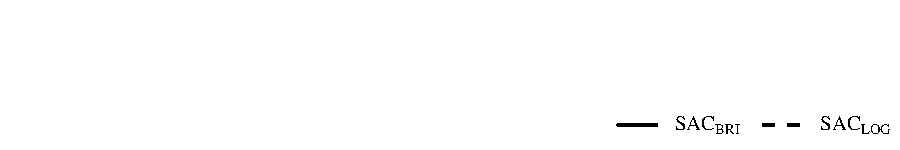
\includegraphics{Figures/LegendSynthetic} % requires the graphicx package
\vspace{-1.5em}

\subfigure{
\hspace{-1em} 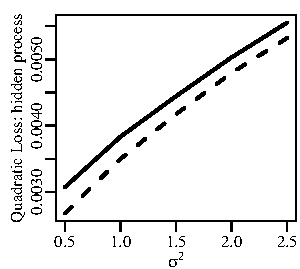
\includegraphics{Figures/SyntheticSigma2}
\label{SyntheticSigma2}
}
\subfigure{
\hspace{-1.5em} 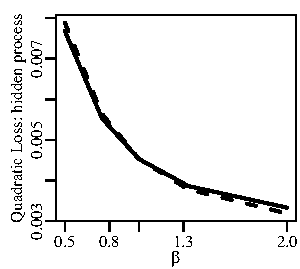
\includegraphics{Figures/SyntheticBeta}
\label{SyntheticBeta}
}
\subfigure{
\hspace{-1.5em} 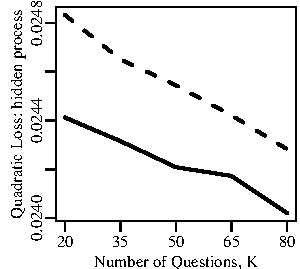
\includegraphics{Figures/SyntheticK}
\label{SyntheticK}
}

\vspace{-1em}

\subfigure{
\hspace{-1em}  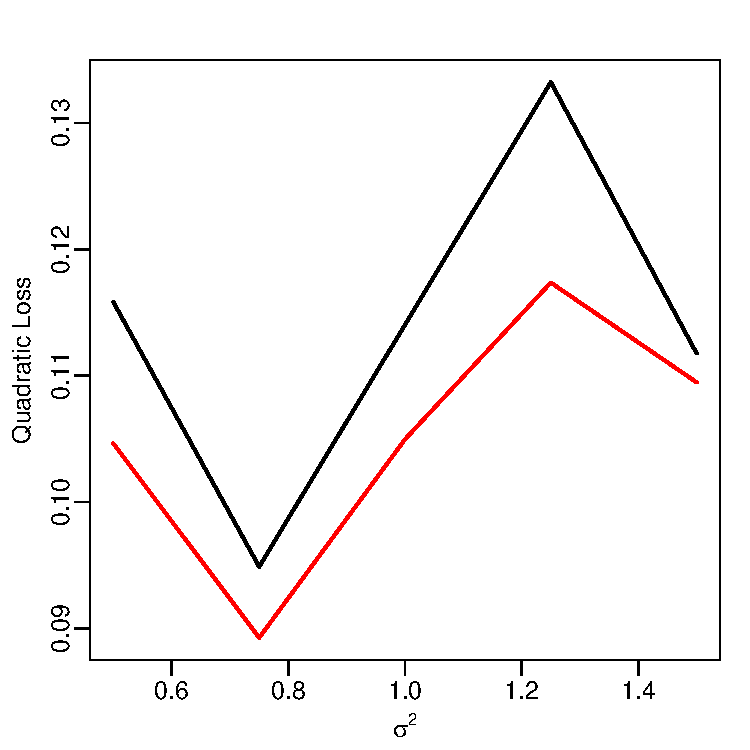
\includegraphics{Figures/SyntheticSigma2bias}
\label{SyntheticSigma2b}
}
\subfigure{
\hspace{-1.5em}  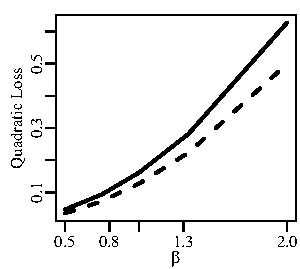
\includegraphics{Figures/SyntheticBetabias}
\label{SyntheticBetab}
}
\subfigure{
\hspace{-1.5em}   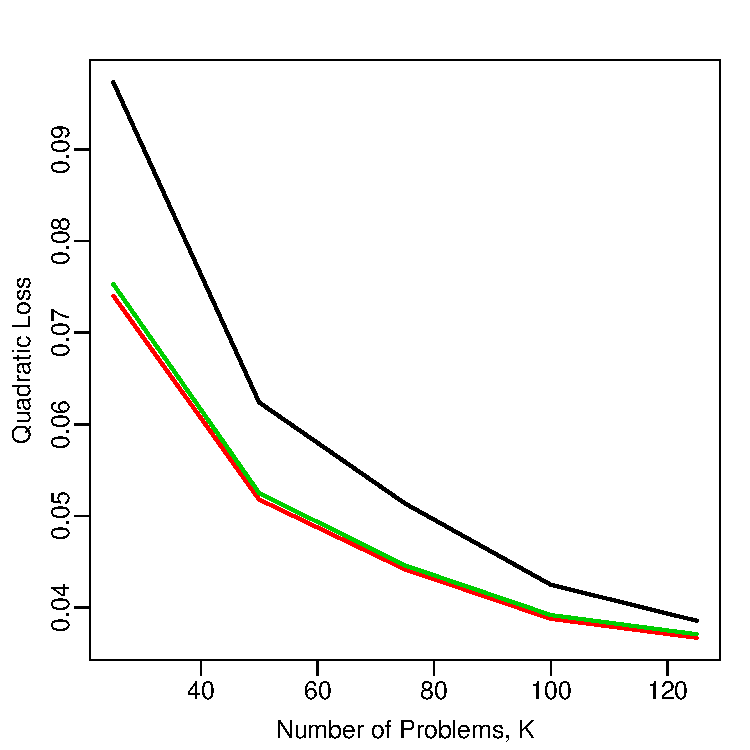
\includegraphics{Figures/SyntheticKbias}
\label{SyntheticKb}
}


\caption[Optional caption for list of figures]{Comparing SAC that optimizes over the logarithmic score ($\text{SAC}_{\text{LOG}}$) and SAC that optimizes over the Brier score ($\text{SAC}_{\text{BRI}}$) under synthetic data. The top row presents the accuracy to capture the hidden process. The bottom row presents the accuracy to capture the bias vector. }
\label{Synthetic}
\end{figure}

Figure \ref{Synthetic} summarizes the results in a series of plots. The first row presents the marginal effects of the three grid variables on the accuracy to which the SAC-procedure estimates the hidden process.  The second row is similar in nature but measures the accuracy in estimating the bias vector instead.  Since the plots were computed by choosing one grid variable (e.g., $\beta$) at a time and averaging over the remaining two variables  (e.g., $K$ and $\sigma^2$), each value in the plots represents an average of a $40 \times 5^2 = 1,000$ values. Based on these results, both $\text{SAC}_{\text{LOG}}$ and  $\text{SAC}_{\text{BRI}}$ estimate the hidden process and the bias vector very accurately. Apart from $\text{SAC}_{\text{LOG}}$ outperforming $\text{SAC}_{\text{BRI}}$ uniformly across all parameter values, the two approaches behave very similarly.  They make great use of the increasing number of questions, suffer slightly from the increasing level of noise in the expert logit-probabilities, and perform better when $\beta$ is large. 

%The latter can be seen as a side-effect of measuring the accuracy an estimated multiplicative factor in the absolute scale. The effect is actually 

%
%Since the hidden state is not explicitly engineered to maximize sharpness subject to calibration, the calibration step in our procedure tends to overestimate $\beta$; that is, the estimated hidden process tends to be a bit sharper (more extreme) than the actual hidden process. 
%
%When $\beta$ is large most of the experts are over-confident. As a result, the sampling step produces an estimated hidden process that is too extreme. This estimate therefore must be pulled back towards zero by the calibration step. If the 
%
%
%The story for the estimating the bias vector is a bit different: the discrepancy between the estimate and the true bias vector may be the same in the log-scale when the $\beta$ is small versus when $\beta$ is large. This, however, translates into much smaller differences in the absolute scale that the differences are ultimately measured in our case. For instance, estimating 1/2 with 3/4 is the same as estimating 2 with 4/3. The difference in the first one is 0.25 while in the second 0.6666667. To make this even worse, the distance is squared which emphasizes large differences. 

%
%Based on the first row of plots, $\text{SAC}_{\text{LOG}}$ and $\text{SAC}_{\text{BRI}}$ estimate the hidden process to a similar accuracy. Even though some relative differences are visible, the loss values are very small in absolute terms, hence suggesting good overall accuracy to capture the hidden process. Estimating the hidden process, however, becomes more difficult as either $\sigma^2$ or $\beta$ gets larger. The latter seems more unintuitive and can be understood better by observing that larger values of $\beta$ lead to more extreme expert logit-probabilities and hence to more frequent truncation. This causes the estimation accuracy to degrade because  a high level of truncation results to a drastic deviation from the model assumptions. Increasing the number of questions improves the estimation accuracy but only very little.
%
%
%Based on the second row of plots, $\text{SAC}_{\text{LOG}}$ and $\text{SAC}_{\text{BRI}}$  capture the bias vector rather precisely as long as the true values of $\beta$ and $\sigma^2$ are not very large. This behavior can be again considered as being caused by the truncation of the extreme expert logit-probabilities. Surprisingly, even though $\text{SAC}_{\text{LOG}}$ is more accurate in estimating the bias vector, it is unable to outperform $\text{SAC}_{\text{BRI}}$ in estimating the hidden process. 
%
%
%




\section{Geopolitical Data Results}
\label{realData}
\noindent
This section presents results related to the real-world data described in Section \ref{data}. The goal is to provide application specific insight by discussing the specific research objectives itemized in Section \ref{intro} and also to evaluate the \textit{Sample-And-Calibrate}-procedure in terms of predictive power and calibration. Before presenting the results, however, we discuss two practical matters that must be taken into account when aggregating real-world  probability forecasts.

\subsection{Incoherent and Imbalanced Data}
\label{practicalMatters}
The first matter regards human experts making probability forecasts of 0.0 or 1.0 even if they are not completely sure of the outcome of the event. For instance, all the 166 questions in our dataset contained both a zero and a one. Transforming such forecasts into the logit-space yields infinities that are highly influential and cause problems in model estimation. To avoid this, \citet{Ariely00theeffects} suggest changing $p = 0.00$ and $1.00$ to $p = 0.02$ and $0.98$, respectively. This is similar to \textit{winsorising} that sets the extreme probabilities to a specified percentile of the data (see, e.g., \citet{hastings1947low} for more details on winsorising).  \citet{Geo}, on the other hand, consider only probabilities that fall within a constrained interval, say $[0.001, 0.999]$, and discard the rest. Since this implies ignoring a portion of the data, we adopt the first approach by truncating $p = 0.00$ and $1.00$ to $p = 0.01$ and $0.99$, respectively.  Our results remain insensitive to the exact choice of truncation as long as this is done in a reasonable manner to keep the extreme probabilities from becoming highly influential in the logit-space.  

The second matter is related to the distribution of the class labels in the data. If the set of occurred events is much larger than the set of events that did not occur (or \textit{vice versa}), the dataset is called \textit{imbalanced}. On such data the modeling procedure can end up over-focusing on the larger class, and as a result, give very accurate forecast performance over the larger class at the cost of performing poorly over the smaller class (see, e.g., \citet{chen2009learning, wallace2012class}). Fortunately, it is often possible to use a well-balanced version of the data. The first step is to find a partition $S_0$ and $S_1$ of the question indices $\{1, 2, \dots, K\}$ such that the equality $\sum_{k \in S_0} T_k  = \sum_{k \in S_1} T_k$ is as closely approximated as possible. This is equivalent to an NP-hard problem known in computer science as the \textit{Partition Problem}:  determine whether a given set of positive integers can be partitioned into two sets such that the sums of the two sets equal to each other (see, e.g., \citet{karmarkar1982differencing, hayes2002easiest}). A simple solution is to use a greedy algorithm that iterates through the values of $T_k$ in descending order, assigning each $T_k$ to the subset that currently has the smaller sum (see, e.g. \citet{kellerer2004knapsack, gent1996phase} for more details on the Partition Problem). After finding a well-balanced partition, the next step is to assign the class labels such that the labels for the questions in $S_x$ are equal to $x$ for $x = 0$ or $1$. Recall from section \ref{calibration_step} that $Z_k$ represents the event indicator associated with the $k$th question. To define a balanced set of indicators $ \tilde{Z}_k$ for all $k \in S_x$, let
\begin{align*}
 \tilde{Z}_k &= x\\
\tilde{p}_{i,t,k} &=  \begin{cases} 
1-p_{i,t,k}, & \text{if } Z_k = 1-x,\\
p_{i,t,k}, & \text{if } Z_k = x,
\end{cases}
\end{align*}
where $i = 1, \dots, I_k$, and $t = 1, \dots, T_k$. The resulting set $$\left\{\left(\tilde{Z}_k, \{\tilde{p}_{i,t,k} | i = 1, \dots, I_k, t = 1, \dots, T_k \}\right) \right\}_{k=1}^K$$ is a balanced version of the data. 
This procedure was used to balance our real-world dataset both in terms of events and time points. The final output splits the events exactly in half ($|S_0| = |S_1| = 83$) such that number of time points in the first and second halves are 8,737 and 8,738, respectively. 


\subsection{Out-of-Sample Forecasting}
\label{forecasting}
This section is motivated by decision-making. 
%For instance, recall our example with an investor who consults a group of experts on a daily basis in order to assess whether a stock index will end up trading above some threshold on a given date. 
The goal is to evaluate the out-of-sample predictive performance of \textit{Sample-And-Calibrate} against several other probability aggregation procedures. The models are allowed to utilize a training set before making predictions on an independent testing set. In order to clarify some of the upcoming notation, let $S_{train}$ and $S_{test}$ be index sets that partition the data into training and testing sets of sizes $|S_{train}| = N_{train}$ and $|S_{test}| = 166 - N_{test}$, respectively. This means that the $k$th question is in the training set if and only if $k \in S_{train}$. The competing models are as follows:


\begin{enumerate}
\item \textit{Simple Dynamic Linear Model (SDLM)}. This is equivalent to the dynamic model from Section \ref{model} but with $\boldsymbol{b} = \boldsymbol{1}$ and $\beta = 1$. Thus,
\begin{eqnarray*}
\boldsymbol{Y}_{t, k} &=&  X_{t, k} + \boldsymbol{v}_{t, k}  \\
X_{t, k} &=& \gamma_k X_{t-1, k} + w_{t, k},
\end{eqnarray*}
where $X_{t,k}$ is the logit-probability used for prediction. Since this model is not hierarchical, estimates of the hidden process can be obtained directly for the questions in the testing set without fitting the model first on the training set. In order to make predictions, the sampler is run for 500 iterations of which the first 200 are used for burn-in. The remaining 300 iterations are thinned by discarding every other observation, leaving a final predictive sample of 150 observations. 

\item \textit{The Sample-And-Calibrate procedure both under the Brier ($\text{SAC}_{\text{BRI}}$) and the logarithmic score ($\text{SAC}_{\text{LOG}}$)}. The model is first fit on the training set by running the sampling step for 3,000 iterations of which the first 500 iterations are used for burn-in. After thinning by only keeping every fifth observation, the calibration step is performed for the remaining 500 observations. The out-of-sample prediction is done by running the sampling step for 500 iterations with each consecutive iteration reading in and conditioning on the next value of $\beta$ and $\boldsymbol{b}$ found during the training period. The first 200 iterations are used for burn-in. The remaining 300 iterations are thinned by discarding every other observation, leaving a final predictive sample of 150 observations. 


\item \textit{A fully Bayesian version of $\text{SAC}_{\text{LOG}}$ ($\text{BSAC}_{\text{LOG}}$)}. Denote the calibrated logit-probabilities and  the event indicators across all $K$ questions with $\boldsymbol{X}(1)$ and $\boldsymbol{Z}$, respectively.  The posterior distribution of $\beta$ conditional on $\boldsymbol{X}(1)$ is given by $p(\beta | \boldsymbol{X}(1), \boldsymbol{Z}) \propto p( \boldsymbol{Z} | \beta, \boldsymbol{X}(1)) p(\beta | \boldsymbol{X}(1))$. Recall that the calibration step under $S_{LOG}$ is equivalent to fitting a logistic regression model with $Z_k$ as the response and $\hat{X}_{k,t}(1)$ as the explanatory variable. Therefore the likelihood for the Bayesian version is
\begin{eqnarray}
p( \boldsymbol{Z} | \beta, \boldsymbol{X}(1)) &\propto& \prod_{k=1}^K \prod_{t=1}^{T_k}  \logit^{-1} \left(X_{k,t}(1)/\beta  \right)^{Z_k} \left( 1-  \logit^{-1} \left( X_{k,t}(1)/\beta  \right) \right)^{1-Z_k} \label{OSE2}
\end{eqnarray}
Similarly to  \citet{gelman2003bayesian}, the prior is chosen to be locally uniform, $p(1/\beta) \propto 1$. Posterior estimates of $\beta$ can be sampled from Equation (\ref{OSE2}) using generic sampling algorithms such as the Metropolis algorithm (\citet{metropolis1953equation}) or slice sampling (\citet{neal2003slice}). Since the sampling procedure conditions on the event indicators, the full conditional distribution of the hidden states is not in a standard form. Therefore the Metropolis algorithm is also used for sampling the hidden states. Predictions are made with the same choices of thinning and burn-in as described under \textit{Sample-And-Calibrate}.


\item Due to the lack of previous literature on dynamic aggregation of expert probability forecasts,  the main competitors are exponentially weighted versions of procedures that have been proposed for static probability aggregation:

\begin{enumerate}

\item \textit{Exponentially Weighted Moving Average (EWMA)}. If 
\begin{eqnarray*}
\bar{p}_{t,k}  = \frac{1}{N_{t,k}} \sum_{i=1}^{N_{t,k}} p_{i,t,k},
\end{eqnarray*}
is the average probability forecast given at time $t$ for the $k$th question, then the EWMA forecasts for the $k$th problem are obtained recursively from
\begin{eqnarray*}
\hat{p}_{t,k}(\alpha) =
\begin{cases}
 \bar{p}_{1,k}, & \text{ for } t  = 1, \\
\alpha \bar{p}_{t,k}  + (1-\alpha) \hat{p}_{t-1,k}(\alpha), & \text{ for } t > 1,
\end{cases}
\end{eqnarray*}
where the input parameter $\alpha$ is learned from the training set by 
\begin{eqnarray*}
\hat{\alpha} &=& \argmin_{\alpha \in [0,1]} \sum_{k \in S_{train}} \sum_{t=1}^{T_k} \left(Z_k - \hat{p}_{t,k}(\alpha) \right)^2
\end{eqnarray*}
 
 
\item  \textit{Exponentially Weighted Moving Logit Aggregator (EWMLA)}. This is a moving version of the aggregator $\hat{p}_G(\boldsymbol{b})$ that was introduced in \cite{satopaa}. If $\boldsymbol{p}_{t,k}$ is a vector collecting all the probability forecasts made for the $k$th question at time $t$, then the EWMLA forecasts are found recursively from
\begin{eqnarray*}
\hat{p}_{t,k}(\alpha, \boldsymbol{b}) =
\begin{cases}
G_{t,k}(\boldsymbol{b} ), & \text{ for } t  = 1, \\
\alpha G_{t,k}(\boldsymbol{b} )  + (1-\alpha) \hat{p}_{t-1,k}(\alpha, \boldsymbol{b}),  & \text{ for } t > 1,
\end{cases}
\end{eqnarray*}
where
\begin{eqnarray*}
G_{t,k}(\nu )  &=& \left( \prod\limits_{i=1}^{N_{t,k}} \left( \frac{p_{i, t, k}}{1-p_{i, t, k}} \right)^{ \frac{\boldsymbol{e}_{i,k}'\boldsymbol{b}}{N_{t,k}}} \right) \Bigg/ \left(1+ \prod\limits_{i=1}^{N_{t,k}} \left( \frac{p_{i, t, k}}{1-p_{i, t, k}} \right)^{\frac{\boldsymbol{e}_{i,k}' \boldsymbol{b}}{N_{t,k}}} \right)
\end{eqnarray*}
The vector $\boldsymbol{b}$ collects the bias terms of the different expertise groups. Therefore it is equivalent to the bias vector found under \textit{Sample-And-Calibrate}. The term $\boldsymbol{e}_{i,k}$ is a vector of length 5 indicating which level of self-reported expertise the $i$th expert in the $k$th question belongs to. For instance, if $\boldsymbol{e}_{i,k} = [0, 1, 0, 0, 0]$, then the expert identifies himself with the expertise level two. The tuning parameters $(\alpha, \boldsymbol{b})$ are learned from the training set by
\begin{eqnarray*}
(\hat{\alpha}, \hat{ \boldsymbol{b}}) &=& \argmin_{ \boldsymbol{b} \in \R^5, \alpha \in [0,1]} \sum_{k \in S_{train}} \sum_{t=1}^{T_k} \left(Z_k - \hat{p}_{t,k}(\alpha,  \boldsymbol{b})\right)^2
\end{eqnarray*}


\item  \textit{Exponentially Weighted Moving Beta-transformed Aggregator (EWMBA)}. The static version of the Beta-transformed  aggregator was introduced in \cite{Ranjan08}. A dynamic version can be obtained by replacing $G_{t,k}(\nu )$ in the EWMLA description with
\begin{eqnarray*}
H_{\nu, \tau} \left( \bar{p}_{t,k}\right),
\end{eqnarray*}
where $H_{\nu, \tau}$ is the cumulative distribution function of the Beta distribution and $\bar{p}_{t,k}$ is the average probability forecast defined under EWMA. The tuning parameters $(\alpha, \nu, \tau)$ are learned from the training set by
\begin{eqnarray*}
(\hat{\alpha}, \hat{\nu}, \hat{\tau}) &=& \argmin_{\nu, \tau > 0\ \alpha \in [0,1]} \sum_{k \in S_{train}} \sum_{t=1}^{T_k} \left(Z_k - \hat{p}_{t,k}(\alpha, \nu, \tau)\right)^2
\end{eqnarray*} 

\end{enumerate}
\end{enumerate}



The competing models are evaluated via a 10-fold cross-validation\footnote{A 5-fold cross-validation was also performed. The results were, however, very similar to the 10-fold cross-validation and hence not presented in the paper.} that first partitions the 166 questions into 10 sets. The partition is chosen such that each of the 10 sets has approximately the same number of questions (16 or 17 questions per set in our case) and the same number of time points (between 1760 and 1764 time points per set in our case). The evaluation then iterates 10 times, each time using one of the 10 sets as the testing set and the remaining 9 sets as the training set. Therefore each question is used nine times for training and exactly once for testing. The testing proceeds sequentially one testing question at a time as follows: First, for a question with a time horizon of $T_k$, make a prediction based on the first two days. Compute the Brier score for the aggregate forecast of the second day. Next make a prediction based on the first three days and  compute the Brier score for the most recent day, namely, the third day. Repeat this process until the prediction is made on all of the $T_k-1$ days. This leads to $T_k-1$ Brier scores per testing question and a total of  17,475 Brier scores across the entire dataset. 


Table \ref{prediction} summarizes different ways to aggregate these scores. The first option, denoted by \textit{Scores by Day}, weighs each question by the number of days the question remained open. This is performed by computing the average of the 17,475 scores. The second option, denoted by \textit{Scores by Problem}, gives each question an equal weight regardless how long the question remained open. This is done by first averaging the scores within a question and then averaging the average scores across all the questions. Both scores can be further broken down into subcategories by considering the length of the questions. The final three columns of Table \ref{prediction} divide the questions into \textit{Short} questions (30 days or fewer), \textit{Medium} questions (between 31 and 59 days), and \textit{Long} Problems (60 days or more). The number of questions in these subcategories were 36, 32 and 98, respectively. The bolded scores indicate the lowest score in each column. The values in the parenthesis quantify the variability in the scores: Under \textit{Scores by Day} the values give the standard errors of all the scores. Under \textit{Scores by Problem}, on other hand, the values represent the standard errors of the average scores of the different questions. 

\begin{table}[htbp]
   \centering
      \begin{tabular}{l llll} % Column formatting, @{} suppresses leading/trailing space
 \multicolumn{5}{ c }{Scores by Day}\\
Model & \multicolumn{1}{ c }{All} & \multicolumn{1}{ c }{Short} & \multicolumn{1}{ c }{Medium} & \multicolumn{1}{ c }{Long}\\ \hline
SDLM & 0.100 (0.156) & 0.066 (0.116) & 0.098 (0.154) & 0.102 (0.157)\\ 
$\text{BSAC}_{\text{LOG}}$ & 0.097 (0.213) & \textbf{0.053} (0.147) & 0.100 (0.215) & 0.098 (0.215)\\ 
$\text{SAC}_{\text{BRI}}$ & 0.096 (0.190) & 0.056 (0.134) & 0.097 (0.190) & 0.098 (0.192)\\ 
$\text{SAC}_{\text{LOG}}$ & \textbf{0.096} (0.191) & 0.056 (0.134) & \textbf{0.096} (0.189) & \textbf{0.098} (0.193)\\ 
EWMBA & 0.102 (0.203) & 0.060 (0.124) & 0.110 (0.201) & 0.103 (0.206)\\ 
EWMLA & 0.102 (0.199) & 0.061 (0.130) & 0.111 (0.214) & 0.103 (0.200)\\ 
EWMA & 0.111 (0.142) & 0.089 (0.100) & 0.111 (0.136) & 0.112 (0.144)\\ 
&&&&\\
\multicolumn{5}{ c }{Scores by Problem}\\
Model & \multicolumn{1}{ c }{All} & \multicolumn{1}{ c }{Short} & \multicolumn{1}{ c }{Medium} & \multicolumn{1}{ c }{Long}\\ \hline
SDLM & 0.089 (0.116) & 0.064 (0.085) & 0.106 (0.141) & 0.092 (0.117)\\ 
$\text{BSAC}_{\text{LOG}}$ & 0.083 (0.160) & \textbf{0.052} (0.103) & 0.110 (0.198) & 0.085 (0.162)\\ 
$\text{SAC}_{\text{BRI}}$& 0.083 (0.142) & 0.055 (0.096) & 0.106 (0.174) & 0.085 (0.144)\\ 
$\text{SAC}_{\text{LOG}}$ & \textbf{0.082} (0.142) & 0.055 (0.096) & \textbf{0.105} (0.174) & \textbf{0.085} (0.144)\\ 
EWMBA & 0.090 (0.156) & 0.063 (0.101) & 0.118 (0.186) & 0.091 (0.161)\\ 
EWMLA & 0.090 (0.159) & 0.064 (0.109) & 0.120 (0.200) & 0.090 (0.159)\\ 
EWMA & 0.104 (0.105) & 0.092 (0.081) & 0.119 (0.125) & 0.103 (0.107)\\ 
   \end{tabular}
   \caption{Brier Scores based on 10-fold cross-validation. \textit{Scores by Day} weighs a question by the number of days the question remained open. \textit{Scores by Problem} gives each question an equal weight regardless how long the question remained open. The bolded values indicate the lowest scores in each column. The values in the parenthesis represent standard errors in the scores. }
   \label{prediction}
\end{table}


Overall, $\text{SAC}_{\text{BRI}}$ and $\text{SAC}_{\text{LOG}}$ achieve the lowest average scores across all columns except \textit{Short}, where they are slightly outperformed by $\text{BSAC}_{\text{LOG}}$.  $\text{BSAC}_{\text{LOG}}$, however, turns out to be overconfident (see Section \ref{calibration}). This means that $\text{BSAC}_{\text{LOG}}$ underestimates the uncertainty in the events and outputs probability forecasts that are typically too near 0.0 or 1.0. As a result, the aggregate forecasts are either very close to the correct answer or very far from it.  As can be seen in Table \ref{prediction}, this results into highly variable forecasting performance. The short questions, however, involve very little uncertainty and were generally the easiest to forecast. On such easy questions, overconfidence can pay off frequently enough to compensate for a few large scores arising from the overconfident and incorrect forecasts. 

In comparison to $\text{BSAC}_{\text{LOG}}$, the baseline SDLM-model lacks sharpness and is highly under-confident (see Section \ref{calibration}). This behavior is expected as the experts are under-confident at the group-level (see Section \ref{ExpertBias}) and the SDLM-procedure does not use the training set to explicitly calibrate its forecasts. Instead, it merely smooths the forecasts given by the experts. The resulting aggregate forecasts are therefore necessarily conservative, resulting into high average scores with low variability. 

 Similarly behavior is exhibited by EWMA that performs the worst of all the competing models. The other two exponentially weighted aggregators, namely EWMLA and EWMBA, on other hand, make efficient use of the training set and present good forecasting performance in most columns of Table \ref{prediction}. Recall that EWMBA uses the cumulative distribution function of the Beta distribution to transform the average forecast probability. This transformation depends on two parameters and is more flexible than the transformation used by EWMLA. On other hand, only EWLMA is given access to the self-reported expertise information. Based on the results, however, it is unable to use this information to outperform EWMBA. Overall, these two aggregators perform very similarly. Unfortunately, they both suffer from over-confidence and are hence unable to outperform the \textit{Sample-And-Calibrate}-procedure.


%The dataset contained a few long questions with an abrupt change of the crowd belief from one answer option to another. Since these abrupt changes happened generally towards the end of each question, during most days the Brier scores were really high. Given that these problems were typically very long, they gained a higher weight under \textit{Scores by Day} than under \textit{Scores by Problem}. This explains why the \textit{Scores by Day} are higher than the \textit{Scores by Problem} under the columns \textit{All Problems} and \textit{Long}.



\subsection{In- and Out-of-Sample Sharpness and Calibration}
\label{calibration}
A calibration plot is a simple tool for visually assessing the sharpness and calibration of a model. The idea is to plot the probability forecasts against the observed empirical frequencies. Therefore any deviation from the diagonal line suggests poor calibration. A model is considered under-confident (or over-confidence) if the points follow an S-shaped (or \reflectbox{S}-shaped) trend. In order to assess sharpness of the model, it is common practice to place a histogram of the given forecasts in the corner of the plot. Since the data were balanced, any deviation from the the baseline probability of 0.5 suggests improved sharpness.



\begin{figure}[h!]
\newgeometry{left=5cm, right = 1cm, bottom=0.1cm}

\subfigure[\scriptsize SDLM In-Sample]{
\hspace*{-3em}  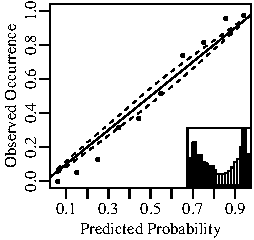
\includegraphics{Figures/CalibrationNONE10}
\label{CalibrationNONEa}
}
\subfigure[\scriptsize $\text{SAC}_{\text{LOG}}$ In-Sample]{
\hspace*{-1.15em} 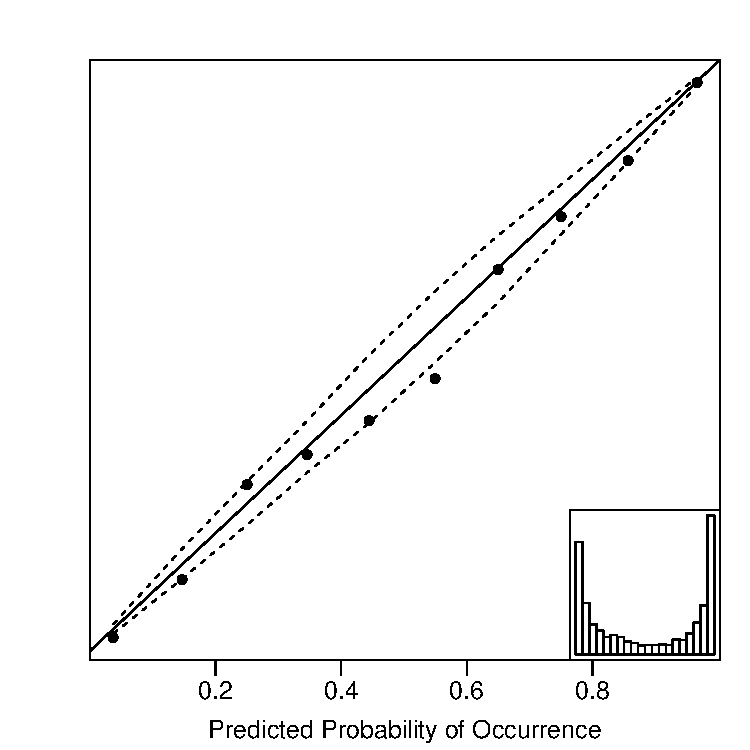
\includegraphics{Figures/CalibrationLOG10}
\label{CalibrationPLATTLOG10}
}
\subfigure[\scriptsize $\text{SAC}_{\text{BRI}}$ In-Sample]{
\hspace*{-1.15em} 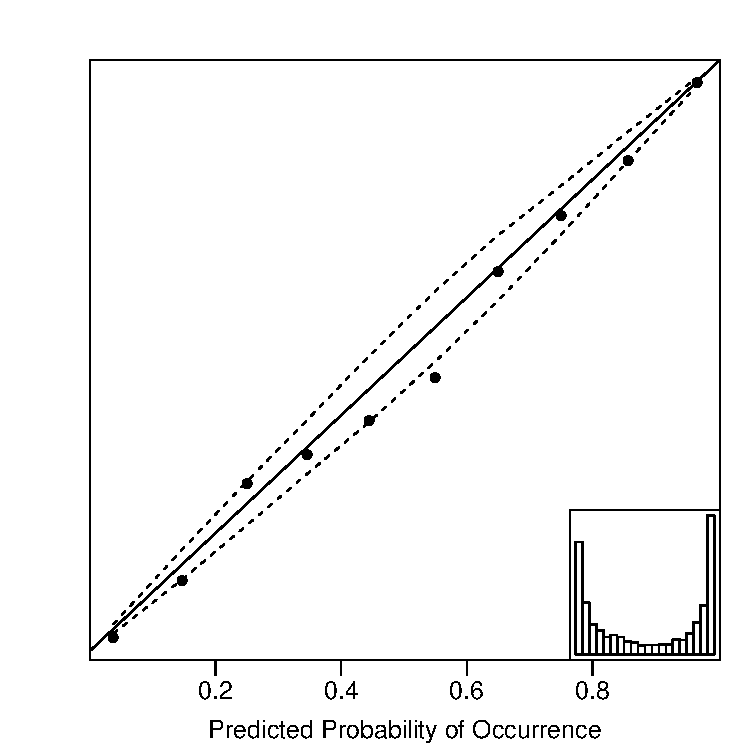
\includegraphics{Figures/CalibrationBRI10}
\label{CalibrationPLATTBRI10}
}
\subfigure[\scriptsize $\text{BSAC}_{\text{LOG}}$ In-Sample]{
\hspace*{-1.15em} 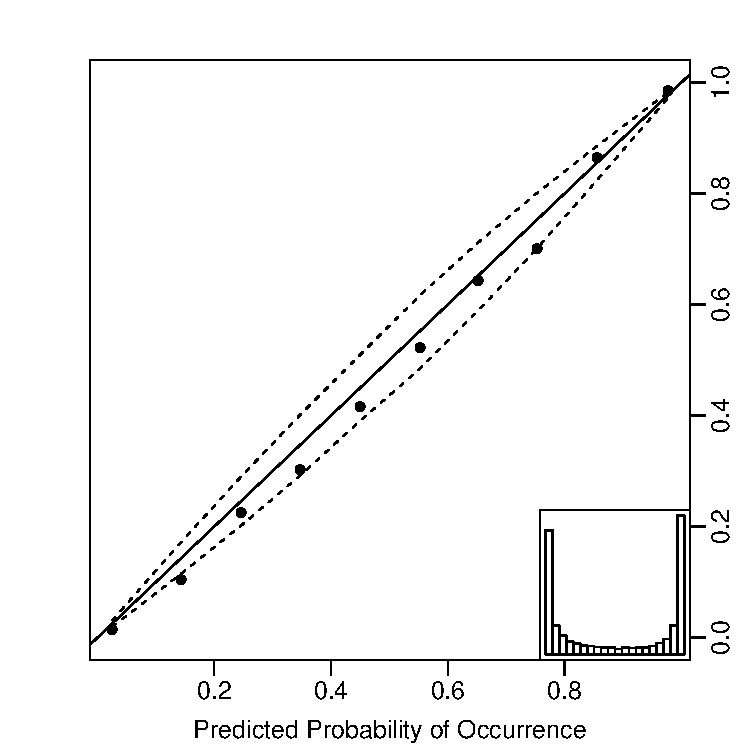
\includegraphics{Figures/CalibrationFULL10}
\hspace*{-2em} \label{CalibrationPLATTFULL10}
}


\subfigure[ \scriptsize SDLM Out-of-Sample]{
\hspace*{-3em} 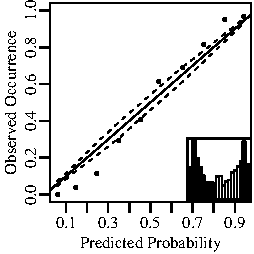
\includegraphics{Figures/CalibrationNONE}
\label{CalibrationNONEb}
}
\subfigure[ \scriptsize $\text{SAC}_{\text{LOG}}$ Out-of-Sample]{
\hspace*{-1.15em} 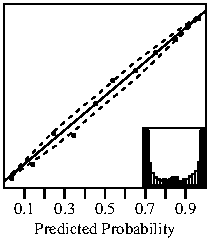
\includegraphics{Figures/CalibrationSTO-Log}
\label{CalibrationSTC-Log}
}
\subfigure[ \scriptsize $\text{SAC}_{\text{BRI}}$ Out-of-Sample]{
\hspace*{-1.15em} 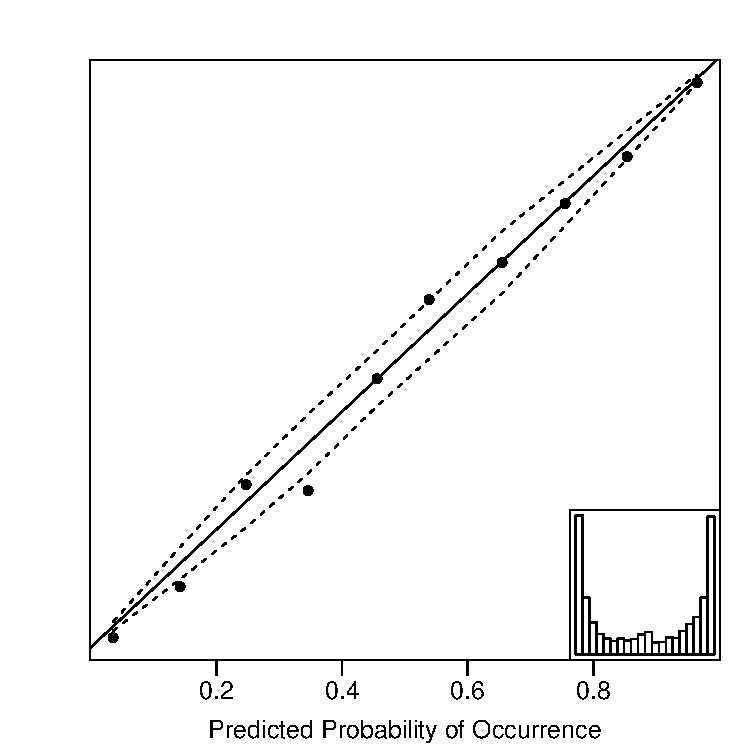
\includegraphics{Figures/CalibrationSTO-Bri}
\label{CalibrationSTC-Bri}
}
\subfigure[\scriptsize  $\text{BSAC}_{\text{LOG}}$ Out-of-Sample]{
\hspace*{-1.15em} 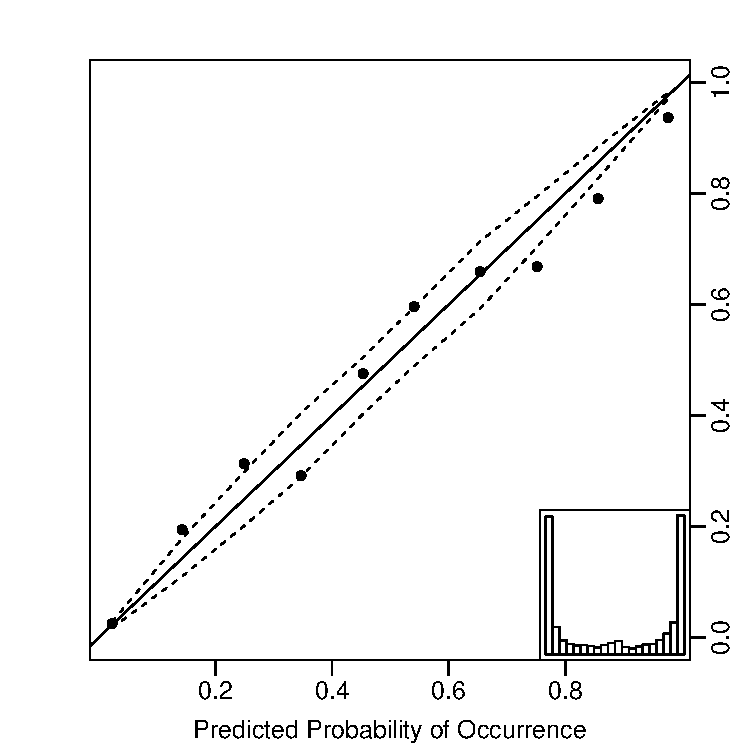
\includegraphics{Figures/CalibrationSO}
\hspace*{-2em}\label{CalibrationBSTC-Log}
}
\restoregeometry
\caption[Optional caption for list of figures]{The top and bottom rows show in- and out-of-sample calibration and sharpness, respectively. The models are Simple Dynamic Linear Model (SDLM), the \textit{Sample-And-Calibrate} approach that optimizes over the logarithmic score ($\text{SAC}_{\text{LOG}}$), the \textit{Sample-And-Calibrate} approach that optimizes over the Brier score ($\text{SAC}_{\text{BRI}}$), and the fully-Bayesian version of the \textit{Sample-And-Calibrate} approach that optimizes over the logarithmic score ($\text{BSAC}_{\text{LOG}}$).
}
\label{Calibration-Out}
\end{figure}


The top and bottom rows of Figure \ref{Calibration-Out} present calibration plots for SDLM, $\text{SAC}_{\text{LOG}}$, $\text{SAC}_{\text{BRI}}$, and $\text{BSAC}_{\text{LOG}}$ under in- and out-of-sample probability estimation, respectively. Each setting is of interest in its own right:  Good in-sample calibration is crucial for model interpretability. In particular, if the estimated crowd belief is well-calibrated, then the elements of the bias vector $\boldsymbol{b}$ can be used to study the amount of under- or over-confidence in the different expertise groups. Good out-of-sample calibration and sharpness, on other hand, are necessary properties in predicting future events with high accuracy.  To guide our assessment, the dashed bands around the diagonal connect the point-wise, Bonferroni-corrected (\citet{bonferroni}) 95\% lower and upper critical values under the null hypothesis of calibration. These have been computed by running the bootstrap technique described in \citet{brocker2007increasing} for 10,000 iterations. The in-sample predictions were obtained by running the models for 10,200 iterations, leading to a final posterior sample of 1,000 observations after thinning and using the first 200 iterations for burn-in. The out-of-sample predictions were given by the 10-fold cross-validation discussed in Section \ref{forecasting}.

Overall, the \textit{Sample-And-Calibrate}-procedure is sharp and well-calibrated both in- and out-of-sample with only a few points barely falling outside the \textit{point-wise} critical values. Since the calibration does not change drastically from the top to the bottom row, the \textit{Sample-And-Calibrate}-procedure can be considered to present robustness against over-fitting. This is, however, not the case with $\text{BSAC}_{\text{LOG}}$ that is well-calibrated in-sample but presents over-confidence out-of-sample. Figures \ref{CalibrationNONEa} and \ref{CalibrationNONEb} serve as baselines by showing the reliability plots for the SDLM-model. Since this model does not perform any explicit calibration, it is not surprising to see most points outside the critical values. The pattern in the deviations suggests drastic under-confidence. Furthermore, the inset histogram reveals drastic lack of sharpness. Therefore the \textit{Sample-And-Calibrate}-model can be viewed as a well-performing compromise between SDLM and $\text{BSAC}_{\text{LOG}}$ that avoids over-confidence without being too conservative. 
 


\subsection{Group-Level Expertise Bias}
\label{ExpertBias}

\begin{figure}[!ht]
\vspace*{-1em} 
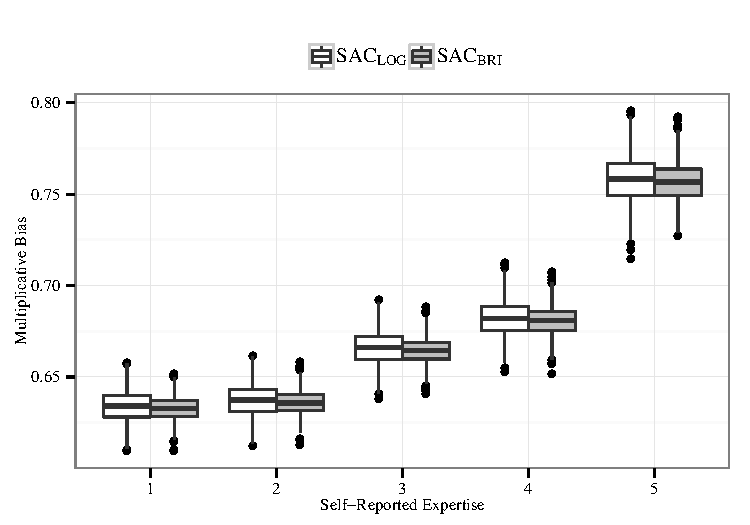
\includegraphics{Figures/BiasesBoxplots}
\label{BiasesLOGBoxplots}
\vspace*{-2em} 

\caption[Optional caption for list of figures]{Comparing the bias-levels across self-reported expertise under different approaches. 
Posterior distributions of $b_j$ for $j = 1, \dots, 5$ under the \textit{Sample-And-Calibrate} approach that optimizes over the logarithmic score and the \textit{Sample-And-Calibrate} approach that optimizes over the Brier score.
}
\label{Biases}
\end{figure}


Recall from Section \ref{data} that the experts were asked to self-assess their level of expertise (on a 1-to-5 scale with 1 = Not At All Expert to 5 = Extremely Expert) on any questions in which they participated. The self-reported expertise then divides the experts into 5  groups, with each group assigned a separate multiplicative bias term. This section uses the \textit{Sample-And-Calibrate}-procedure to explore the posterior distributions of these multiplicative bias terms. Figure \ref{Biases} presents the posterior distributions of the bias terms with side-by-side box plots. Since the distributions fall completely below the \textit{no-bias} reference-line at 1.0, all the groups are deemed under-confident. Even though the exact level of under-confidence is affected slightly by the extent to which the extreme probabilities are truncated (see Section \ref{practicalMatters}), the qualitative results in this section remain insensitive to different levels of truncation. 



The under-confidence decreases as the level of  expertise increases.  For instance, the posterior probability that the most expert group is the least under-confident is approximately equal to $1.0$, and the posterior probability of a strictly decreasing level of under-confidence is approximately 0.87. The latter probability is driven down by the inseparability of the two groups with the lowest levels of self-reported expertise. The fact that these groups are very similar suggests that the experts are poor at assessing how little they know about a subject that is strange to them. If these groups are combined into a single group, the posterior probability of a strictly decreasing level of under-confidence is approximately 1.0. 

The decreasing trend in under-confidence can be reasoned by viewing the process of making a subjective probability  as Bayesian updating: A completely ignorant expert aiming to minimize a reasonable loss function, such as the Brier score, has no reason to give anything but 0.5 as his probability forecast. However, as soon as the expert gains some knowledge about the event, he produces an updated forecast that is a compromise between his initial forecast and the new information acquired. The updated forecast is therefore conservative and too close to 0.5 as long as the expert remains only partially informed about the event. If most experts fall somewhere on this spectrum between ignorance and full information, their average forecast tends to fall strictly between 0.5 and the most-informed probability forecast (see \citet{Baron} for more details). Since expertise is to a large extent determined by subject-matter knowledge, the level of under-confidence can be expected to decrease as a function of the group's level of self-reported expertise.

Finding under-confidence in all the groups is a rather surprising result given that many previous studies have been conducted to show that experts are likely to be over-confident. For instance,  \citet{lichtenstein1977calibration, morgan1992uncertainty, bier2004implications} summarize the results from numerous calibration studies, and conclude that experts are systematically over-con�dent about their probability assessments. Our result, however, is a statement about groups of experts and hence does not invalidate the possibility of the individual experts being overconfident. To make conclusions at the individual-level based on the group-level bias terms would be considered an \textit{ecological inference fallacy} (see, e.g., \citet{lubinski1996seeing}).



%More specific group-level inference can be performed by computing probabilities based the estimated posterior distributions. For instance, the posterior probability that the most expert group is the least under-confident is approximately equal to $1.0$, and 
%the posterior probability of a strictly decreasing level of under-confidence by expertise ranking is approximately 0.87. The latter probability is driven down by the inseparability of the two groups associated with the lowest levels of self-reported expertise. The fact that these groups are very similar suggests that the experts are poor at assessing how little they know about a subject that is strange to them. If these groups are combined into a single group, the posterior probability of a strictly decreasing level of under-confidence is approximately 1.0. 








\subsection{Question Difficulty and Other Measures}
\label{QuestionDifficulty}
One advantage of our model arises from its ability to produce estimates of interpretable question-specific parameters $\gamma_k$, $\sigma^2_k$, and $\tau^2_k$. These quantities can be combined in many interesting ways to answer questions about different groups of experts or the questions themselves. For instance, being able to assess the difficulty of a question could lead to more principled ways of aggregating performance measures across questions or to novel insight on the kind of questions that are found difficult by experts (see, e.g., a discussion on the \textit{Hard-Easy Effect} in \cite{Wilson94cognitivefactors}). To illustrate, recall that higher values of $\sigma^2_k$ suggest greater disagreement among the participating experts. Since experts are more likely to disagree over a difficult question than an easy one, it is reasonable to assume that $\sigma^2_k$ has a positive relationship with question difficulty. An alternative measure is given by $\tau_k$ that quantifies the volatility of the underlying circumstances that ultimately decide the outcome of the event. Therefore a high value of $\tau_k$ can cause the outcome of the event appear unstable and difficult to predict. 


\begin{figure}[h!]
\vspace{-1em}
\centering
\hspace*{0em} 	
\includegraphics{Figures/LegendExamplePlot} % requires the graphicx package
\vspace{-3.5em}

\hspace{-0.5em}
\subfigure[\textit{Will the expansion of the European bailout fund be ratified by all 17 Eurozone nations before 1 November 2011?}]{
\hspace*{-1em}  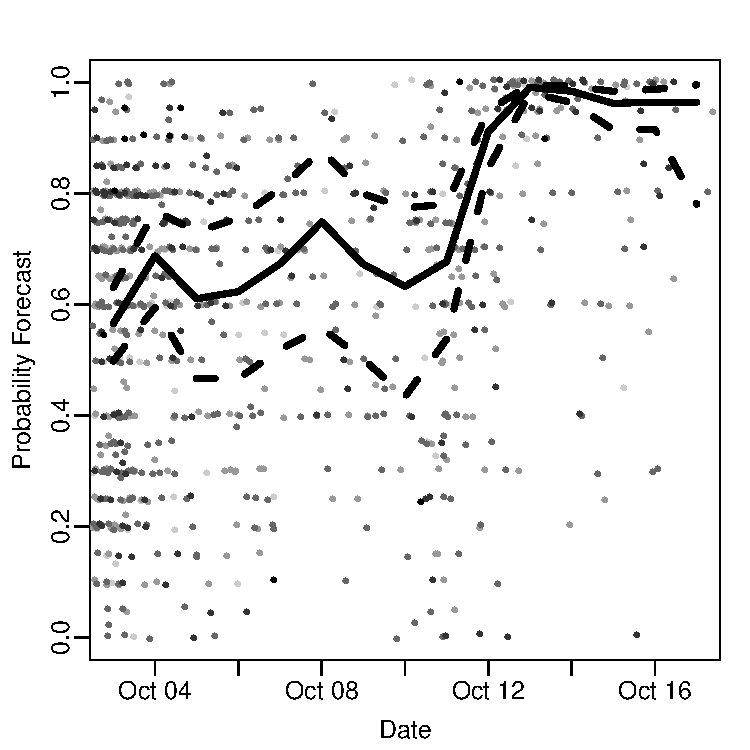
\includegraphics{Figures/ExamplePlot1b}
\label{Example1b}
} \hspace{0.5em}
\subfigure[\textit{Will the Nikkei 225 index finish trading at or above 9,500 on 30 September 2011?}]{
\hspace*{-1em}  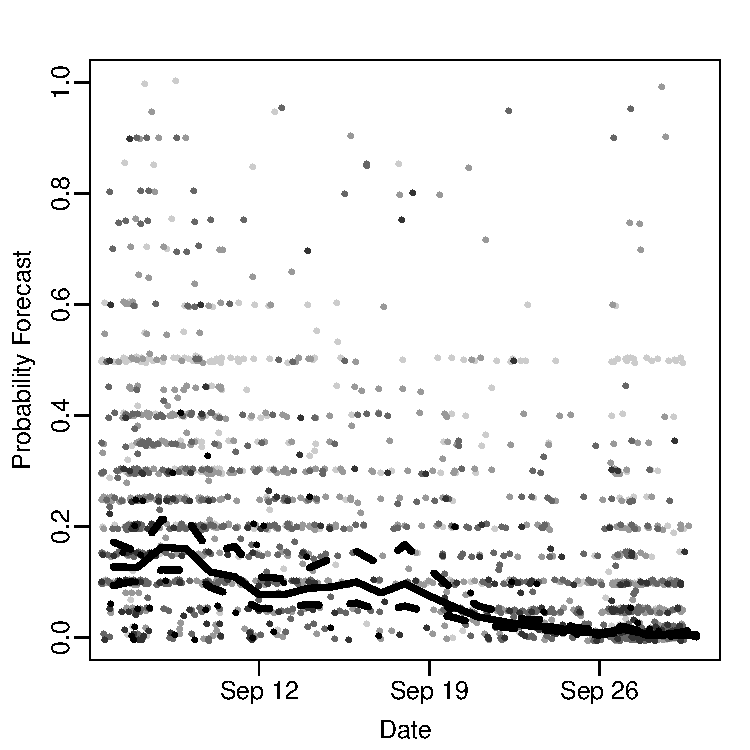
\includegraphics{Figures/ExamplePlot2b}
\label{Example2b}
}

\caption[Optional caption for list of figures]{Scatterplots of the probability forecasts given for two questions in our dataset. The shadings represents the self-reported expertise of the expert who provided the probability forecast. The solid line gives the posterior mean of the calibrated crowd belief as estimated by $\text{SAC}_{\text{LOG}}$. The surrounding dashed lines connect the point-wise 95\% posterior intervals.}
\label{ExamplePlotsFinal}
\end{figure}


As a final illustration of our model, we return to the two example questions introduced in Section \ref{data}. Figure \ref{ExamplePlotsFinal} is a copy of Figure \ref{ExamplePlots} with the addition of a solid line surrounded by a dashed band. The solid line represents the posterior mean of the calibrated crowd belief as estimated by $\text{SAC}_{\text{LOG}}$. The dashed lines connect the point-wise 95\% posterior intervals across different time points. Since $\hat{\sigma}_k^2 = 2.43$  and $\hat{\sigma}_k^2 = 1.77$ for the questions depicted in Figures \ref{Example1b} and \ref{Example2b}, respectively, the first question provokes more disagreement among the experts than the second one. Intuitively this makes sense because the target event in Figure \ref{Example1b}  is determined by several conditions that may change radically from one day to the next while the target event in Figure \ref{Example2b} is determined by a relatively steady stock market index. Therefore it is not surprising to find that in Figure \ref{Example1b} $\hat{\tau}_k^2 = 0.269$, which is much higher than $\hat{\tau}_k^2 = 0.039$ in Figure \ref{Example2b}. We may conclude that the first question is inherently more difficult than the second one. 


\section{Discussion}
This paper began with an introduction of a rather unorthodox but nonetheless realistic time-series setting where probability forecasts are made very infrequently by a heterogeneous group of experts. The resulting data is too sparse to be modeled well with standard time-series methods.  In response to this lack of appropriate modeling procedures, our work introduces an interpretable time-series model that incorporates self-reported expertise to capture a sharp and well-calibrated estimate of the crowd belief. The model estimation is performed in two steps: The first step, known as the \textit{sampling step}, samples constrained versions of the model parameters via Gibbs sampling. The sampling is done from standard distributions with fast convergence to the target distribution (see Appendix \ref{appendix} for technical details). The second step, known as the \textit{calibration step}, uses a one-dimensional optimization procedure to transforms the constrained parameter values to their unconstrained counterparts. To the best of our knowledge, this procedure extends forecasting literature towards rather unexplored areas of probability aggregation.

\subsection{Summary of Findings}
The model was applied to an unusually large dataset on expert probability forecasts. The estimated crowd belief was found to be sharp and well-calibrated under both in- and out-of-sample settings. This has direct implications  on predictive power and model interpretability. First, the model was shown to outperform other probability aggregators in terms of forecasting ability. In particular, the model was deemed a well-balanced compromise that avoids over-fitting without being overly conservative. Second, the crowd belief was used as the no-bias reference point to study the bias among groups of experts with different levels of self-reported expertise. All the groups were found to be under-confident. The under-confidence, however, decreased as the level of self-reported expertise increased. This result is about groups of experts and hence does not conflict with the well-known result of the individuals being over-confident (see, e.g.,  \citet{lichtenstein1977calibration, morgan1992uncertainty, bier2004implications}). Besides making predictions or studying group-level bias, the model can be used to generate estimates of many problem-specific parameters. These quantities have clear interpretations and can be combined in many interesting ways to explore a range of hypotheses about different types of questions and expert behavior. 


\subsection{Limitations and Directions for Future Research}
Our model pertains model parsimony while addressing the main challenges that arise from modeling sparse probability forecasting data. Therefore it can be viewed as a basis for many future extensions. To give some ideas, recall that most of the model parameters were assumed constant over time. It is intuitively reasonable, however, that these parameters behave differently during different time intervals of the question.  For instance, the level of disagreement (represented by $\sigma^2_k$ in our model) among the experts can be expected to decrease towards the final time point when the question  resolves. This hypothesis could be explored by letting $\sigma^2_{t,k}$ evolve dynamically as a function of the previous term $\sigma^2_{t-1,k}$ and random noise. 

If the experts were asked to provide personal information during the data collection process, it may be of interest to study the forecasting behavior of different kinds of experts. For instance, this paper modeled the bias separately within each expertise group. This, however, is by no means restricted to the study of bias or its relation to self-reported expertise. Different parameter dependencies could be constructed based on many other expert characteristic, such as gender, education, or specialty, to produce a range of novel insight on the forecasting behavior across different groups of experts. Furthermore, expert characteristics could be interacted with question types, such as economic, domestic, or international, to learn about the kind of experts who generally perform well on certain types of questions. This would be of interest to the decision-maker who could use the information as a basis for consulting only a high-performing subset of the available experts. 
 
Other future directions could aim to remove some of the obvious limitations of our model. For instance, recall that the random components are assumed to follow a normal distribution. This is a strong assumption that may not always be justified. Logit-probabilities, however, have been modeled with the normal distribution before (see, e.g., \citet{Erev1994}). Furthermore, the normal distribution is a rather standard assumption in psychological models (see, e.g.,  signal-detection theory  in \citet{tanner1954decision}). A second limitation resides in the assumption that both the observed and hidden processes are expected to grow linearly. This assumption could be relaxed, for instance, by adding higher order terms to the model. A more complex model, however, is likely to sacrifice interpretability. Given that our model is able to detect very intricate patterns in the crowd belief  (see Figure \ref{ExamplePlotsFinal}), compromising interpretability for the sake of facilitating non-linear growth is hardly necessary. 


\appendix
\section{Technical Details of the Sampling Step}
\label{appendix}

The Gibbs sampler (\citet{geman1984stochastic}) iteratively samples all the unknown parameters from their full-conditional posterior distributions one block of parameters at a time. Since this is performed under the constraint $b_3 = 1$ to ensure model identifiability, the constrained parameter estimates should be denoted with a trailing $(1)$ to maintain consistency with earlier notation. For instance, the constrained estimate of $\gamma_k$ should be denoted by $\hat{\gamma}_k(1)$ while the unconstrained estimate is denoted by $\hat{\gamma}_k$. For the sake of clarity, however, the constraint suffix is omitted in this section. Nonetheless, it is important to keep in mind that all the estimates in this section are constrained.

\begin{center}
\framecolorbox[\textwidth]{gray}{gray!15}{Sample $X_{t,k}$}
\end{center}
The hidden states are sampled via the \textit{Forward-Filtering-Backward-Sampling} (FFBS) algorithm that first predicts the hidden states using a Kalman Filter and then performs a backward sampling procedure that treats these predicted states as additional observations (see, e.g., \cite{carter1994gibbs, migon2005dynamic} for details on FFBS). More specifically, the first part, namely the Kalman Filter, is deterministic and consists of a predict and an update step. Given all the other parameters except the hidden states, the predict step for the $k$th question is
\begin{align*}
X_{t|t-1,k} &= \gamma_k X_{t-1|t-1,k} \\
P_{t|t-1, k} &= \gamma_k^2 P_{t-1|t-1, k} + \tau_k^2,
\end{align*}
where the initial values, $X_{0|0,k}$ and $P_{0|0, k}$, are equal to $0$ and $1$, respectively. The update step is 
\begin{align*}
e_{t,k} &= Y_{i,t,k} - b_{i,k} X_{t | t-1, k} \\
S_{t,k} &=  \sigma_k^2 + b_{i,k}^2 P_{t|t-1, k}\\
K_{t,k} &=  P_{t|t-1, k} b_{i,k} S_{t,k}^{-1} \\
X_{t|t, k} &= X_{t|t-1, k} + K_{t,k} e_{t,k} \\
P_{t|t,k} &= (1 - K_{t,k} b_{i,k}) P_{t|t-1,k},
\end{align*}
where $b_{i,k}$ is the corresponding bias term for the $i$th expert in the $k$th question. The update step is repeated sequentially for each observation $Y_{i,t,k}$ given at time $t$. For each such repetition of the update step, the previous posterior values, $X_{t|t, k}$ and $P_{t|t, k}$, should be considered as the new prior values, $X_{t|t-1, k}$ and $P_{t|t-1, k}$. After running the Kalman Filter up to the final time point at $t = T_k$, the final hidden state is sampled from $X_{T_k,k} \sim \mathcal{N}(X_{T_k|T_k, k}, P_{T_k|T_k, k})$. The remaining states are obtained via the backward sampling that is performed in reverse from
\begin{align*}
X_{t-1, k} &\sim  \mathcal{N} \left(V\left( \frac{\gamma_kX_{t,k}}{\tau_k^2}  + \frac{X_{t|t,k}}{P_{t|t,k} } \right),  V\right),
\end{align*}
where
\begin{align*}
V &= \left( \frac{\gamma_k^2}{\tau_k^2} + \frac{1}{P_{t|t,k}}\right)^{-1}
\end{align*}
This can be viewed as backward updating that considers the Kalman Filter estimates as additional observations at each given time point. If the observation $\boldsymbol{Y}_{t,k}$ is completely missing at time $t$, the update step is skipped and the state estimates are sampled from
\begin{align*}
\mathcal{N}\left(\gamma_k X_{t-1|t-1,k}, \gamma_k^2 P_{t-1|t-1,k} + \tau_k^2\right)
\end{align*}

\begin{center}
\framecolorbox[\textwidth]{gray}{gray!15}{Sample $\boldsymbol{b}$ and $\sigma^2_k$}
\end{center}
First, vectorize all the response vectors $\boldsymbol{Y}_{t,k}$ into a single vector denoted $\boldsymbol{Y}_k = \left[\boldsymbol{Y}_{1,k}^T, \dots, \boldsymbol{Y}_{T_k,k}^T\right]^T$. Since each $\boldsymbol{Y}_{t,k}$ is matched with $X_{t,k}$ via the time index $t$, we can form a $|\boldsymbol{Y}_k| \times J$ design-matrix by letting $\boldsymbol{X}_k = \left[ (\boldsymbol{M}_kX_{1,k})^T, \dots, (\boldsymbol{M}_kX_{T_k,k})^T \right]^T$. Given that the goal is to borrow strength across questions by assuming a common bias vector $\boldsymbol{b}$, the parameter values must be estimated in parallel for each question such that the matrices $\boldsymbol{X}_k$ can be further concatenated into $\boldsymbol{X} = [\boldsymbol{X}_1^T, \dots, \boldsymbol{X}_K^T]^T$ during every iteration. Similarly, $\boldsymbol{Y}_k$ must be further vectorized into a vector $\boldsymbol{Y} = [\boldsymbol{Y}_1^T, \dots, \boldsymbol{Y}_K^T]^T$. The question-specific variance terms are taken into account by letting $\boldsymbol{\Sigma} = \text{diag}(\sigma^2_1 \boldsymbol{1}_{1 \times T_1}, \dots, \sigma^2_K \boldsymbol{1}_{1 \times T_K})$.  After adopting the non-informative prior $p(\boldsymbol{b}, \sigma_k^2 | \boldsymbol{X}_k) \propto \sigma_k^{-2}$ for each $k = 1, \dots, K$, the bias vector are sampled from
\begin{eqnarray}
\boldsymbol{b} | \dots &\sim& \mathcal{N}_J \left( (\boldsymbol{X}^T \boldsymbol{\Sigma}^{-1} \boldsymbol{X})^{-1} \boldsymbol{X}^T \boldsymbol{\Sigma}^{-1} \boldsymbol{Y}, (\boldsymbol{X}^T \boldsymbol{\Sigma}^{-1} \boldsymbol{X})^{-1} \right) \label{BiasVector}
\end{eqnarray}
Since the covariance matrix in Equation (\ref{BiasVector}) is diagonal, the constraint is enforced at this point by letting $b_3 = 1$. The variance parameter is then sampled from
\begin{eqnarray*}
\sigma^2_k | \dots &\sim& \text{Inv-}\chi^2\left(|\boldsymbol{Y}_k| - J, \frac{1}{|\boldsymbol{Y}_k| - J} (\boldsymbol{Y}_k - \boldsymbol{X}_k \boldsymbol{b})^T (\boldsymbol{Y}_k - \boldsymbol{X}_k \boldsymbol{b}) \right),
\end{eqnarray*}
where the distribution is a scaled inverse-$\chi^2$ (see, e.g., \citet{gelman2003bayesian}). Since the experts are not required to give a new prediction at every time unit, the design matrices must be trimmed accordingly such that their dimensions match up with the dimensions of the observed matrices. 


\begin{center}
\framecolorbox[\textwidth]{gray}{gray!15}{Sample $\gamma_k$ and $\tau^2_k$}
\end{center}
Estimating the parameters related to the hidden process are estimated via a regression setup. More specifically, after adopting the non-informative prior $p(\gamma_k, \tau_k^2 | \boldsymbol{X}_k) \propto \tau_k^{-2}$, the parameter values are sampled from
\begin{eqnarray*}
\gamma_k | \dots  &\sim&  \mathcal{N} \left( \frac{\sum_{t=2}^{T_k} X_{t,k}X_{t-1,k}}{\sum_{t=1}^{T_k-1} X_{t,k}^2} , \frac{\tau_k^2}{\sum_{t=1}^{T_k-1} X_{t,k}^2} \right)\\
\tau_k^2 | \dots &\sim& \text{Inv-}\chi^2 \left(T_k-1, \frac{1}{T_k-1} \sum_{t=2}^{T_k} \left(X_{t,k} - \gamma_k X_{t-1,k} \right)^2 \right),
\end{eqnarray*}
where the final distribution is a scaled inverse-$\chi^2$ (see, e.g., \citet{gelman2003bayesian}).


\bibliographystyle{imsart-nameyear}
\bibliography{biblio}		% expects file "myrefs.bib"


\end{document}